\documentclass[9pt]{beamer}
%\documentclass[9pt,aspectratio=169]{beamer}
\usepackage[utf8]{inputenc}
\usepackage[english]{babel}
\usepackage[T1]{fontenc}
\usepackage{tikz}
\usepackage{times}
\usefonttheme[onlymath]{serif} 
\usepackage{etoolbox}
\usepackage{xcolor}
\usepackage{amsmath}
\usepackage{graphicx}
\usepackage{pdfpages}
\usepackage[absolute,overlay]{textpos}
\usepackage{animate}
\usepackage{booktabs}
\usepackage{verbatim}
\usepackage{biblatex}
\usepackage{tikz}
\usepackage{media9}
\addbibresource{dlpbibli.bib}

% Defining new colors
\definecolor{DarkGreen}{rgb}{0.0, 0.65, 0.31}
\definecolor{NewRed}{rgb}{0.89, 0.02, 0.17}


\usetheme{ARMINES}

\author[Daniella LOPES PINTO]{Daniella LOPES PINTO \textsuperscript{1,2*} \\ 
\texttt{\textcolor{black}{daniella.lopes\_pinto@minesparis.psl.eu}}}
\subtitle{\LARGE Finite element models for the study of hydrogen embrittlement of steel structures}

\institute
{\textbf{Academic advisor}: Jacques BESSON \textsuperscript{1} \\
\vspace{0.25cm}
\textbf{Industrial advisors}: Nikolay OSIPOV \textsuperscript{2} \\
\vspace{0.4cm}
{\textsuperscript{1} Centre des Matériaux, Mines Paris} \\
\vspace{0.15cm}
\textsuperscript{2} Transvalor S.A. \\
\vspace{0.2cm}
\center{\textbf{Thesis defense} \\ \small March 7\textsuperscript{th} 2025} 
\center{\textcolor{white}{XXXXXXXX}}}


\begin{document}

\begin{frame}[plain]
    \maketitle
\end{frame}

\section{Introduction}

%%%%%%%%%%%%%%%%%%%%%%%%%%%%%%%%%%%%%%%%%%%%%%%%%%%%%%%%%%%

\begin{frame}{Background and challenges}

    \begin{itemize}
		\item In the context of \textbf{energy transition}, \textbf{hydrogen} plays an important role as an \textbf{energy vector}
		\vspace{0.15cm}
		\item Hydrogen can be produced from other \textbf{renewable sources}, such as wind and solar
		\vspace{0.15cm}
		\item Hydrogen transport using \textbf{existing natural gas pipelines} (40,000 km in France, €50 billion in assets, up to 80 years old) is a proposal for hydrogen transport
    \end{itemize}
    
    \vspace{0.2cm}

\begin{figure}
	\centering
	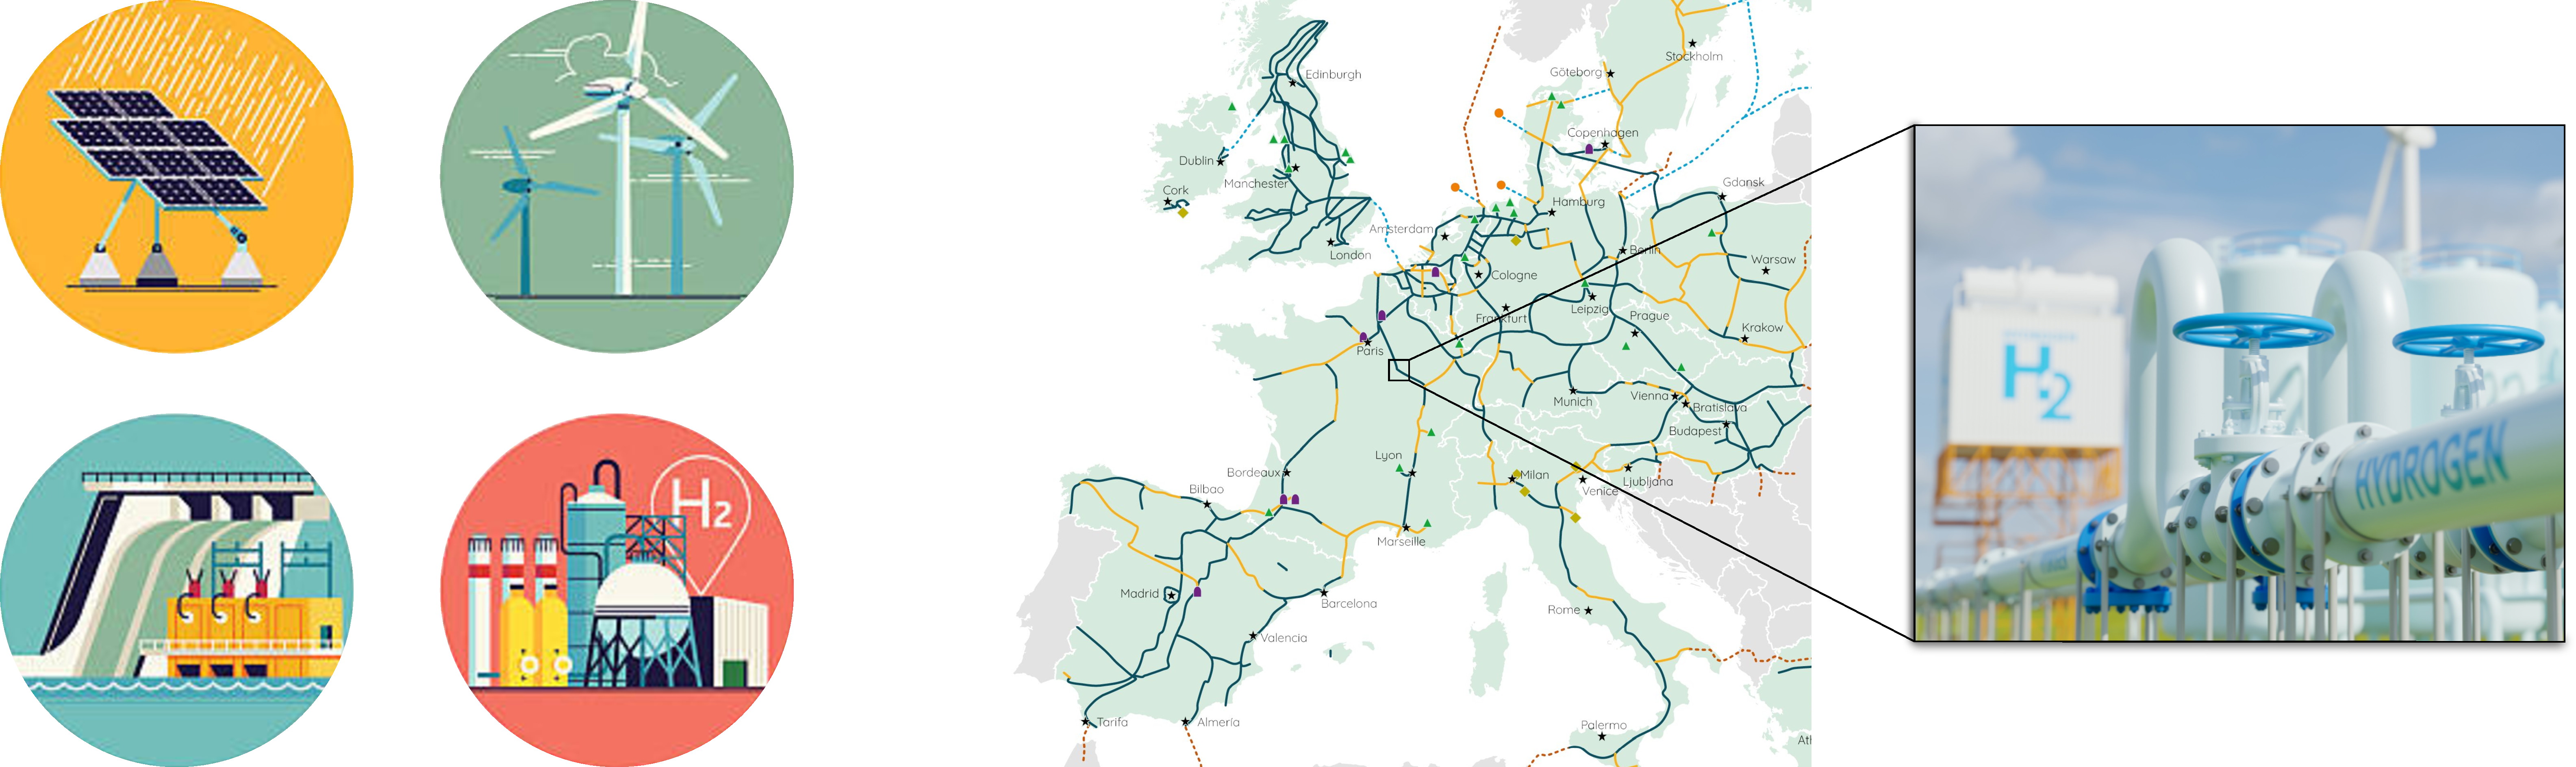
\includegraphics[width=0.92\textwidth]{Images/Context.pdf}
\end{figure}
    
\end{frame}

%%%%%%%%%%%%%%%%%%%%%%%%%%%%%%%%%%%%%%%%%%%%%%%%%%%%%%%%%%%

\begin{frame}{Background and challenges}

\begin{itemize}
	\item The steels used in gas pipelines are typically susceptible to \textbf{hydrogen embrittlement}
	\vspace{0.15cm}
	\item Hydrogen embrittlement: ductility and toughness reduction, premature failure
	\vspace{0.15cm}
	\item \textbf{Measure material properties from small samples without service interruption}
\end{itemize}

\vspace{0.15cm}

\begin{figure}
	\centering
	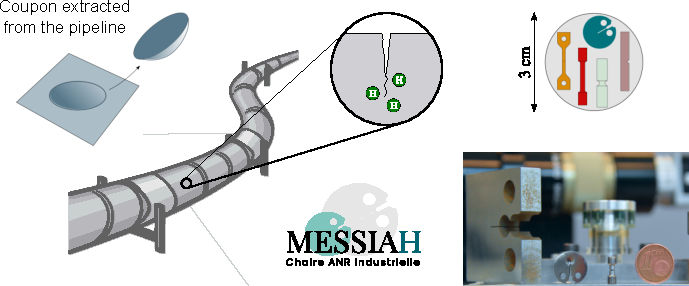
\includegraphics[width=0.95\textwidth]{Images/MESSIAH.pdf}
\end{figure}

\end{frame}

%%%%%%%%%%%%%%%%%%%%%%%%%%%%%%%%%%%%%%%%%%%%%%%%%%%%%%%%%%%

\begin{frame}{Background and Challenges}

\begin{itemize}
    \item Experimental observations show that \textbf{toughness decreases with increasing specimen thickness} until reaching a plateau
    \vspace{0.15cm}
    \item Beyond a critical thickness, toughness becomes relatively insensitive to further increases
\end{itemize}

\begin{figure}
    \centering
    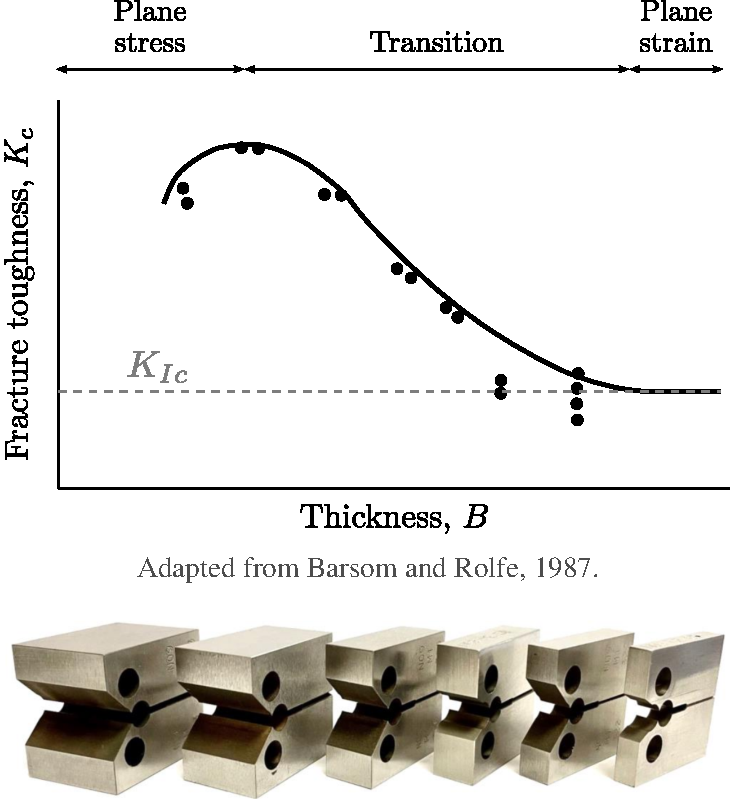
\includegraphics[width=0.75\textwidth]{Images/plateau_plane_strain.pdf}
\end{figure}


\end{frame}

%%%%%%%%%%%%%%%%%%%%%%%%%%%%%%%%%%%%%%%%%%%%%%%%%%%%%%%%%%%

\begin{frame}{Main objectives}

\begin{itemize}
    \item Develop a model coupling \textbf{plasticity}, \textbf{damage}, and \textbf{hydrogen diffusion}
    \vspace{0.15cm}
    \item Validate the model against experimental data
    \vspace{0.15cm}
    \item Simulate size and thickness effects on toughness using sub-size specimens
\end{itemize}

% Say that this model not only allows the prediction of hydrogen assisted failure, but also to estimate the hydrogen distribution during loading and it can help interpreting experiments
% Add figures and animations from TISD ?

\end{frame}

%%%%%%%%%%%%%%%%%%%%%%%%%%%%%%%%%%%%%%%%%%%%%%%%%%%%%%%%%%%

\begin{frame}{Outline}
    \tableofcontents
\end{frame}

%%%%%%%%%%%%%%%%%%%%%%%%%%%%%%%%%%%%%%%%%%%%%%%%%%%%%%%%%%%%

\section{Hydrogen inside metals}

\begin{frame}{Outline}
	\tableofcontents[ 
    currentsubsection, 
    hideothersubsections, 
    sectionstyle=show/shaded, 
    subsectionstyle=show/shaded, 
    ] 
\end{frame}

%%%%%%%%%%%%%%%%%%%%%%%%%%%%%%%%%%%%%%%%%%%%%%%%%%%%%%%%%%%

\begin{frame}{Hydrogen uptake}

\begin{itemize}
	\item \textbf{Sieverts' law:} The solubility of a diatomic gas in a metal is proportional to the square root of the gas pressure
\end{itemize}

\vspace{1cm}

    \begin{minipage}{0.55\textwidth}
        \centering
        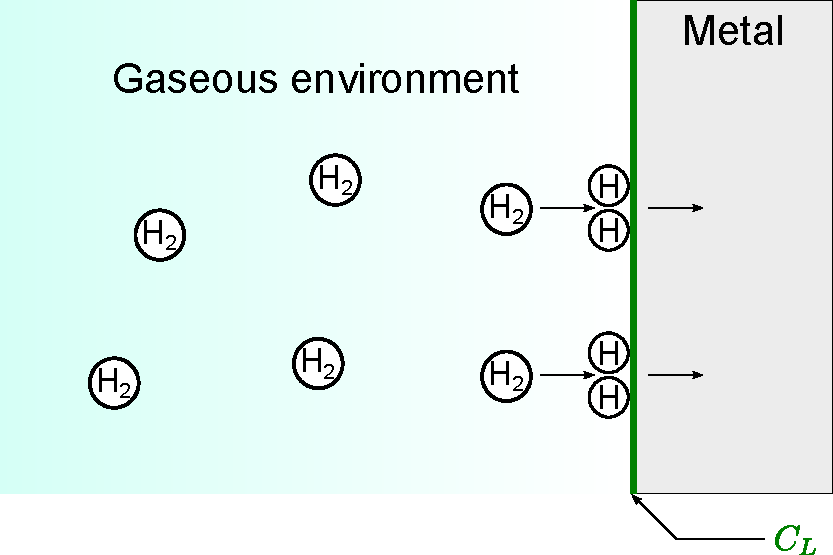
\includegraphics[width=\textwidth]{Images/H2_uptake.pdf}
    \end{minipage}
    \hfill
    \begin{minipage}{0.42\textwidth}
        \centering
        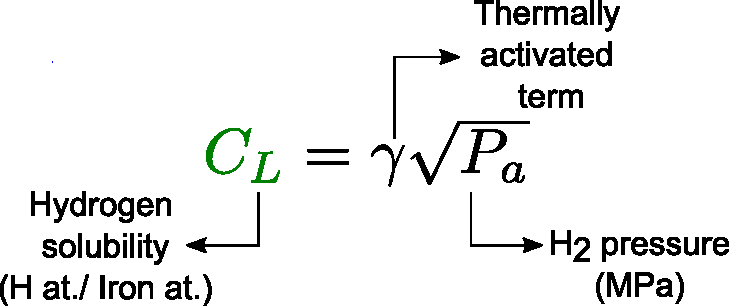
\includegraphics[width=\textwidth]{Images/sieverts.pdf}
    \end{minipage}

\end{frame}

%%%%%%%%%%%%%%%%%%%%%%%%%%%%%%%%%%%%%%%%%%%%%%%%%%%%%%%%%%%

\begin{frame}{Hydrogen diffusion and trapping}

    \begin{columns}
    
        \begin{column}{0.8\textwidth}
    
            \begin{itemize}
                \item Model from \textcolor{darkgray}{Sofronis and McMeeking (1989)} and corrected by \textcolor{darkgray}{Krom \textit{et al.} (1999)}
                
                \vspace{0.35cm}
            
                \item \textbf{Hydrogen concentration:} \hspace{0.5cm} $ \displaystyle C = \textcolor{DarkGreen}{C_L} + \textcolor{blue}{C_T}$
    
                \begin{itemize}
                    \vspace{0.35cm}
                    \item Lattice concentration: \hspace{1.0cm} $\displaystyle \textcolor{DarkGreen}{C_L} = \beta N_L \theta_L$
                    
                    \vspace{0.35cm}
        
                    \item Trapped concentration: \hspace{0.1cm} $\displaystyle \textcolor{blue}{C_T} = \sum_i^N C_T^i = \textcolor{NewRed}{N_T^i(\kappa)} \theta_T^i$
    
                \end{itemize}
    
                \vspace{0.35cm}
    
                \item \textbf{Hydrogen flux:}
    
                \begin{equation*}
                    J = -D_L \nabla \textcolor{DarkGreen}{C_L} + \frac{D_L \textcolor{DarkGreen}{C_L} V_H}{RT} \textcolor{NewRed}{\nabla p}
                \end{equation*}
            
                \vspace{0.1cm}
            
                \item \textbf{Oriani's equilibrium:}
                
                \begin{equation*}
                    \frac{1- \theta_L}{\theta_L} \frac{\theta_T^i}{1- \theta_T^i} = K
                \end{equation*}
                  
            \end{itemize}
    
            \vspace{0.3cm}
            
        \end{column}
        
        \begin{column}{0.2\textwidth}
        \end{column}
        
	\end{columns}
	
	\begin{tikzpicture}[remember picture, overlay]
    	\node at (current page.south west) [xshift=9.5cm, yshift=6cm] {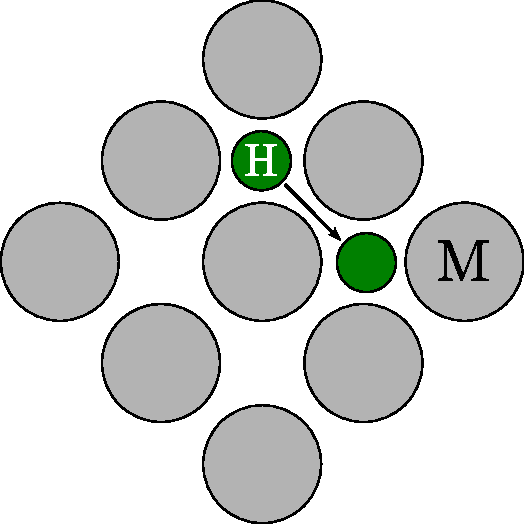
\includegraphics[width=2.5cm]{Images/CL.pdf}}; 
    \end{tikzpicture}
    
    \begin{tikzpicture}[remember picture, overlay]
		\node at (current page.south west) [xshift=10cm, yshift=2.5cm] {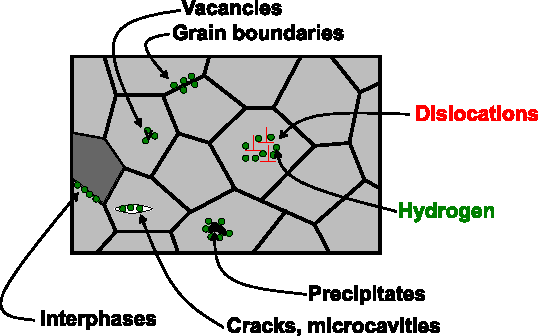
\includegraphics[width=4.5cm]{Images/CT.pdf}}; 
	\end{tikzpicture}
     
	\begin{textblock}{5}(1,14.)
        \textcolor{NewRed}{\footnotesize (Coupling terms)}
    \end{textblock}

\end{frame}

%%%%%%%%%%%%%%%%%%%%%%%%%%%%%%%%%%%%%%%%%%%%%%%%%%%%%%%%%%%

\begin{frame}{Material damage}

    \begin{itemize}
        \item The \textbf{ductile behavior} of the metal is described by the \textbf{GTN model} (\textcolor{darkgray}{Tvergaard \textit{et al.} 1984}):
     \end{itemize}

        $$ \displaystyle \frac{\sigma_{eq}^2}{\sigma_F^2} + 2 q_1 f_* \cosh \left(\frac{q_2}{2} \frac{\sigma_{ii}}{\sigma_F}\right) - 1 -q_1^2 f_*^2 = 0 $$ 

        \vspace{0.15cm}

        $$ \displaystyle \dot{f} = \dot{f}_{nucleation} + \dot{f}_{growth} $$

        \vspace{0.15cm}

        \begin{figure}
            \centering
            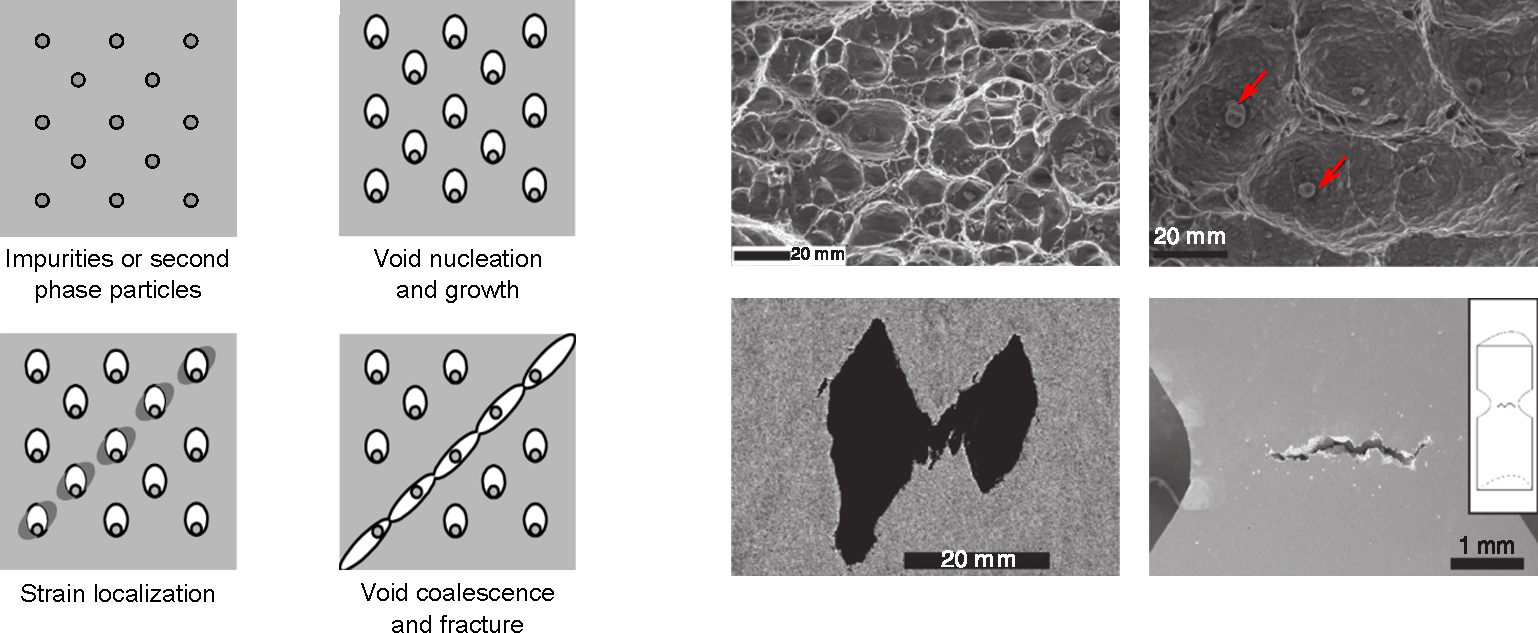
\includegraphics[width=0.9\textwidth]{Images/damage_evolution.pdf}
        \end{figure}
        
\end{frame}

%%%%%%%%%%%%%%%%%%%%%%%%%%%%%%%%%%%%%%%%%%%%%%%%%%%%%%%%%%%

\begin{frame}{Hydrogen embrittlement}

    \begin{itemize}

        \item \textbf{Void growth}: Unchanged due to mass conservation
        
        \begin{equation*}
            \dot{f}_g = (1-f_g) \textrm{trace}(\dot{\varepsilon}_p)
        \end{equation*}  

        \vspace{0.2cm} 
        
        \item\textbf{Void nucleation}: Proposed dependance on hydrogen concentration
        
        \begin{equation*}
            \dot{f}_n = A_n (\kappa) \dot{\kappa} + \textcolor{NewRed}{B_n (C)} \dot{\kappa}
        \end{equation*}

    \end{itemize}
    
    \hspace{1.5cm} 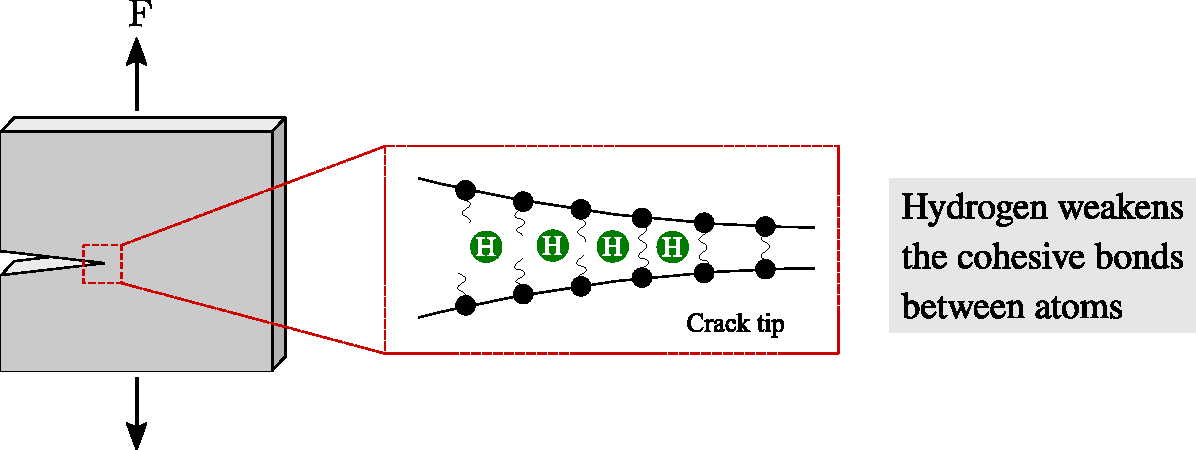
\includegraphics[width=0.75\textwidth]{Images/HEDE3.pdf}

    \begin{textblock}{10}(5,13.5)
        \textcolor{NewRed}{$B_n (C)$}: Damage nucleation due to hydrogen \\ \textbf{HEDE} (Hydrogen Enhanced Decohesion)
    \end{textblock}
    
    \begin{textblock}{5}(13.,7.5)
        \textcolor{NewRed}{\footnotesize (Coupling terms)}
    \end{textblock}

\end{frame}

%%%%%%%%%%%%%%%%%%%%%%%%%%%%%%%%%%%%%%%%%%%%%%%%%%%%%%%%%%%

\section{Finite element formulation}

\begin{frame}{Outline}
	\tableofcontents[ 
    currentsubsection, 
    hideothersubsections, 
    sectionstyle=show/shaded, 
    subsectionstyle=show/shaded, 
    ] 
\end{frame}

%%%%%%%%%%%%%%%%%%%%%%%%%%%%%%%%%%%%%%%%%%%%%%%%%%%%%%%%%%%

\begin{frame}{Mixed formulation}

    \begin{itemize}
        \item Fully implicit finite strain framework
        \vspace{0.1cm}
        \item Based on a mixed formulation: $\underline{u}, P, \theta$ (\textcolor{darkgray}{Zhang \textit{et al.} 2017}) and $C_L$ 
        \vspace{0.1cm}
        \item Quadratic elements with reduced integration
        \vspace{0.1cm}
        \item \textbf{Aim:} better pressure fields by avoiding volumetric locking
    \end{itemize}

    \begin{block}{\textbf{Advantage}}
        $\textcolor{NewRed}{\nabla p}$ can be directly computed from nodal values
        \begin{equation*}
            J = {-D_L \nabla C_L} + {{\frac{D_L C_L V_H}{RT} \textcolor{NewRed}{\nabla p}}}
        \end{equation*} 
    \end{block}
    
    \vspace{0.1cm}
    
    \begin{figure}
        \centering
        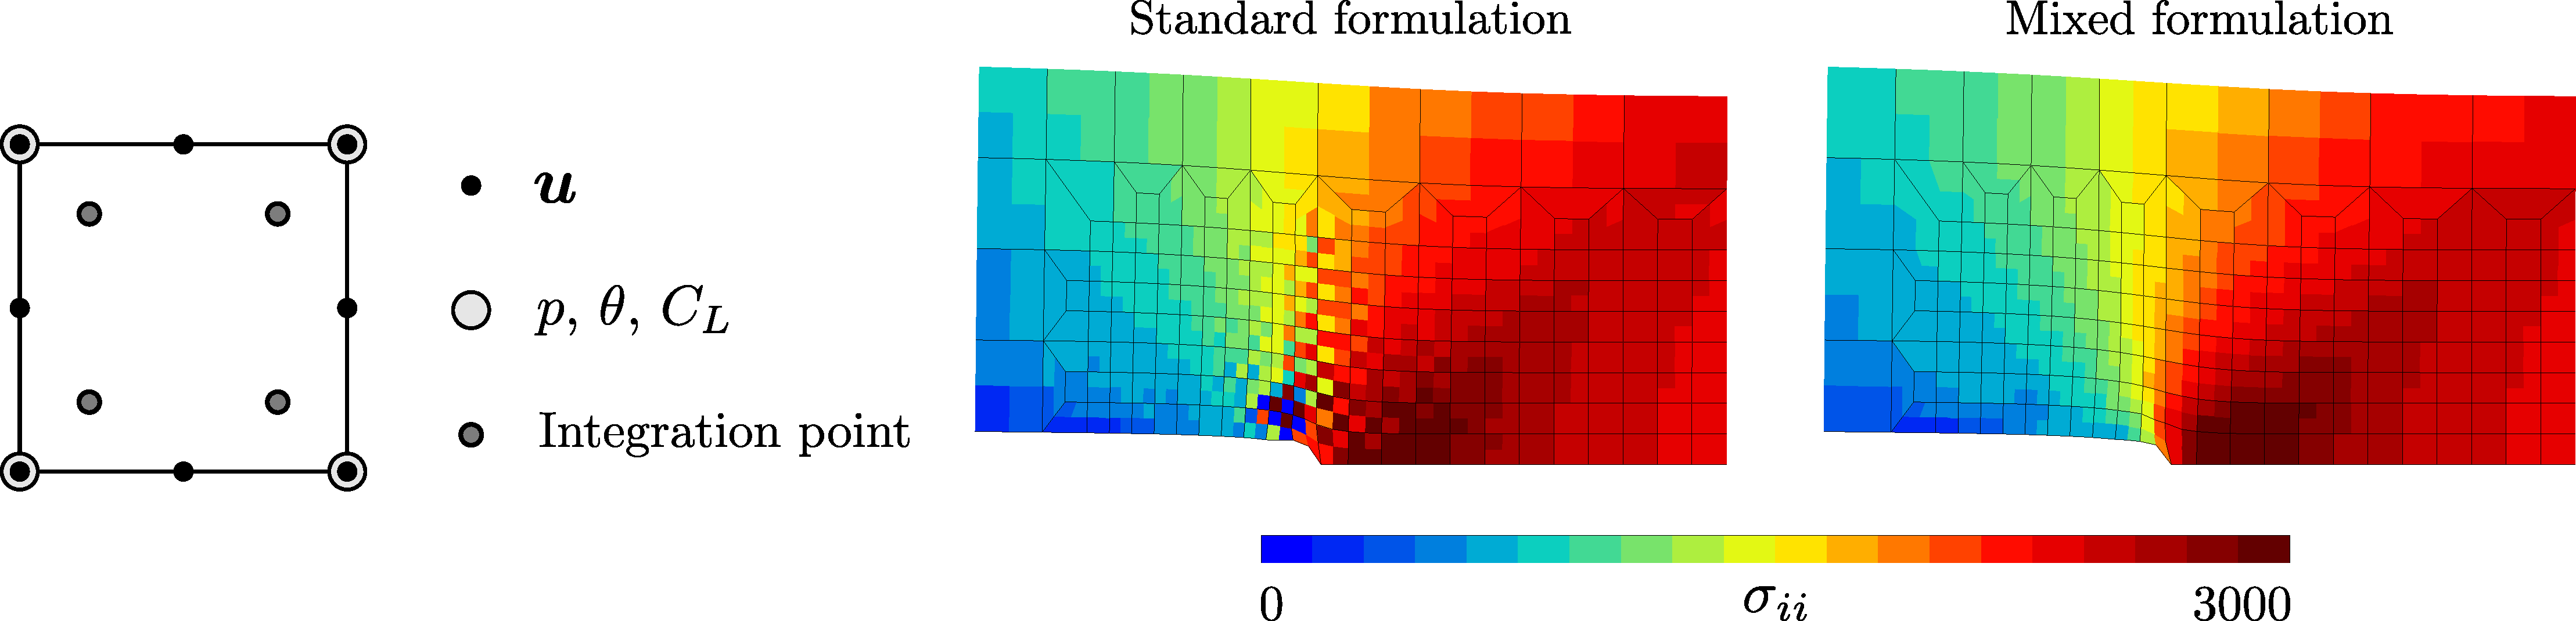
\includegraphics[width=1.\textwidth]{Images/volumetric_locking.pdf}
    \end{figure}

    \begin{tikzpicture}[remember picture, overlay]
        \node at (current page.south west) [xshift=11.5cm, yshift=7.5cm] {
\includegraphics[width=2cm]{Images/Zset.jpg}}; 
    \end{tikzpicture}

\end{frame}

%%%%%%%%%%%%%%%%%%%%%%%%%%%%%%%%%%%%%%%%%%%%%%%%%%%%%%%%%%%

\begin{frame}{$\boldsymbol{B}$-bar formulation}
    
	\begin{itemize}
		\item The use of \textbf{quadratic elements} with additional dofs lead to \\ \textbf{high simulation times}
		\vspace{0.25cm}
		\item $\boldsymbol{B}$-bar (or $\boldsymbol{\bar{B}}$) formulation (\textcolor{darkgray}{Hughes, 1980}): 
		\vspace{0.25cm}
		\begin{itemize}
			\item Linear elements with full integration
			\vspace{0.25cm}
			\item Solves volumetric locking by modifying the strain-displacement matrix: \\
			$$\boldsymbol{\bar{B}} = \boldsymbol{B}_d + \boldsymbol{\bar{B}}_h$$
			\vspace{0.05cm}
			\item To avoid extrapolating $p$ to the nodes for $\nabla p$ computation, it is considered as a dof
		\end{itemize}
	\end{itemize}	
	
	\vspace{0.25cm}	
	
	\begin{figure}
        \centering
        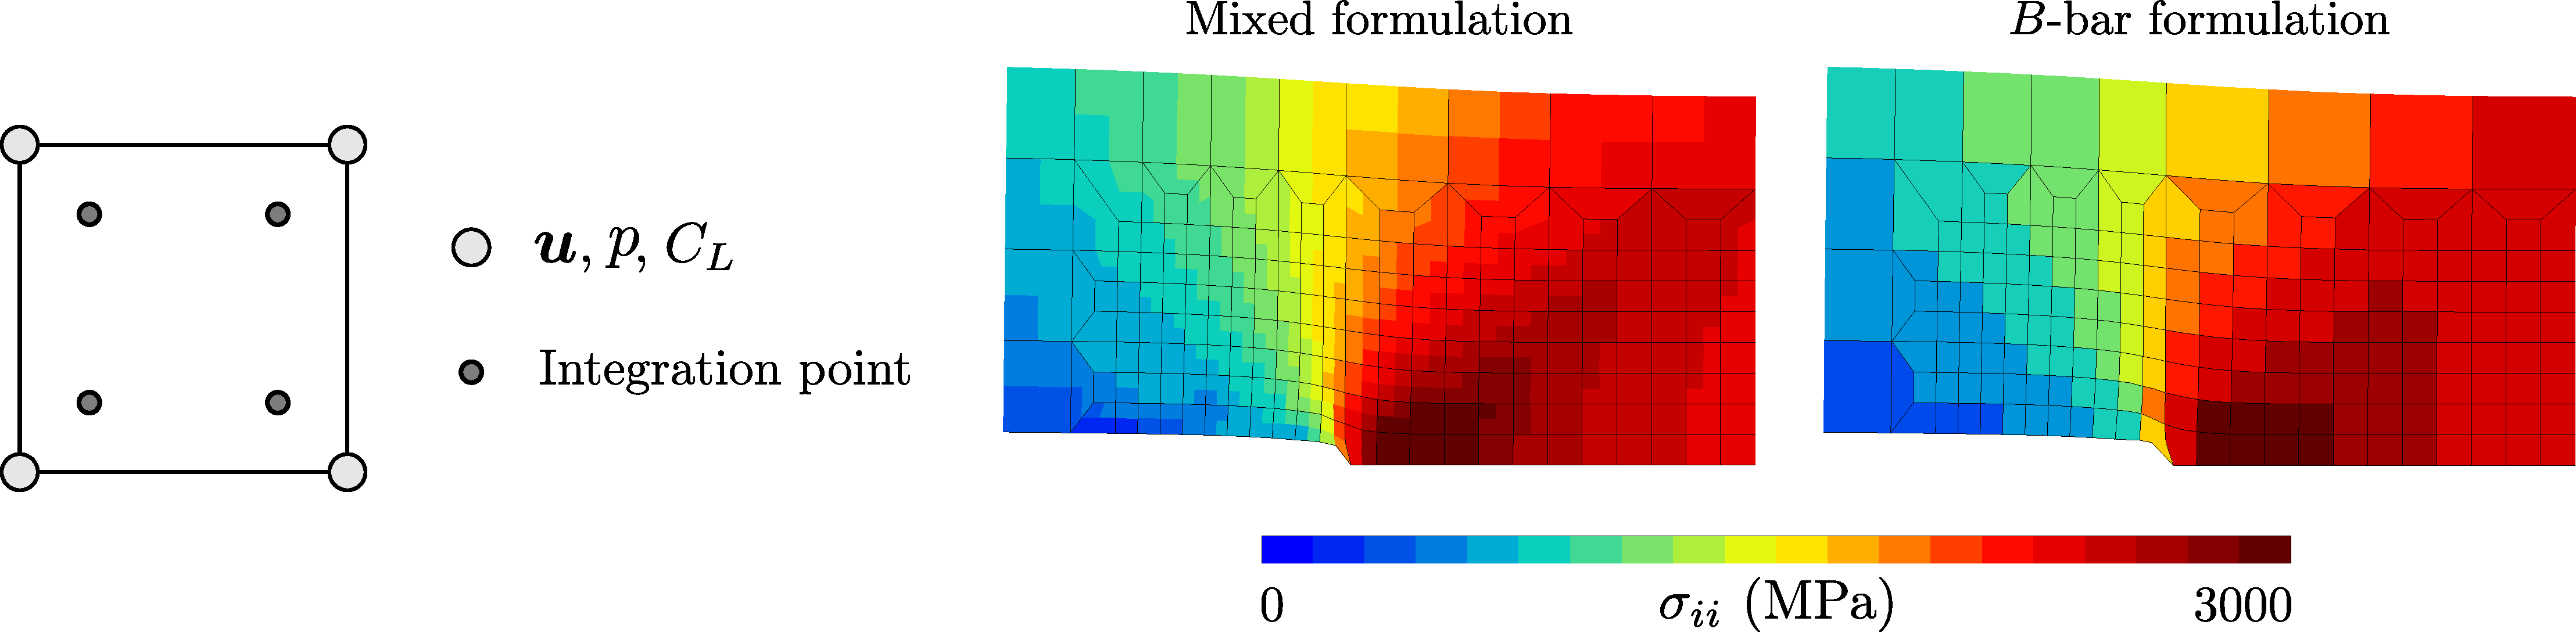
\includegraphics[width=1.\textwidth]{Images/comp_nlgeom-3f_B-bar.pdf}
    \end{figure}  
    
    \begin{tikzpicture}[remember picture, overlay]
        \node at (current page.south west) [xshift=11.5cm, yshift=7.5cm] {
\includegraphics[width=2cm]{Images/Zset.jpg}}; 
    \end{tikzpicture}  
    
\end{frame}

%%%%%%%%%%%%%%%%%%%%%%%%%%%%%%%%%%%%%%%%%%%%%%%%%%%%%%%%%%%

\begin{frame}{$\boldsymbol{B}$-bar formulation}

	\begin{itemize}
		\item Test on a Disk Compact Tension (DCT) specimen with 5200 elements:
		\vspace{0.25cm}
		
		\begin{itemize}
			\item \textbf{Mixed formulation}: 103,762 dofs, 1h 40 minutes to complete
			\vspace{0.25cm}
			\item $\boldsymbol{B}$\textbf{-bar formulation}: 33,974 dofs, 18 minutes to complete
		\end{itemize}
		\vspace{0.25cm}
		\item Slightly higher force for the $\boldsymbol{B}$-bar formulation $\rightarrow$ Linear elements are inherently stiffer since they have less nodes  
	\end{itemize}
	
\begin{columns}
	\begin{column}{0.5\textwidth}
		\begin{figure}
        \centering
        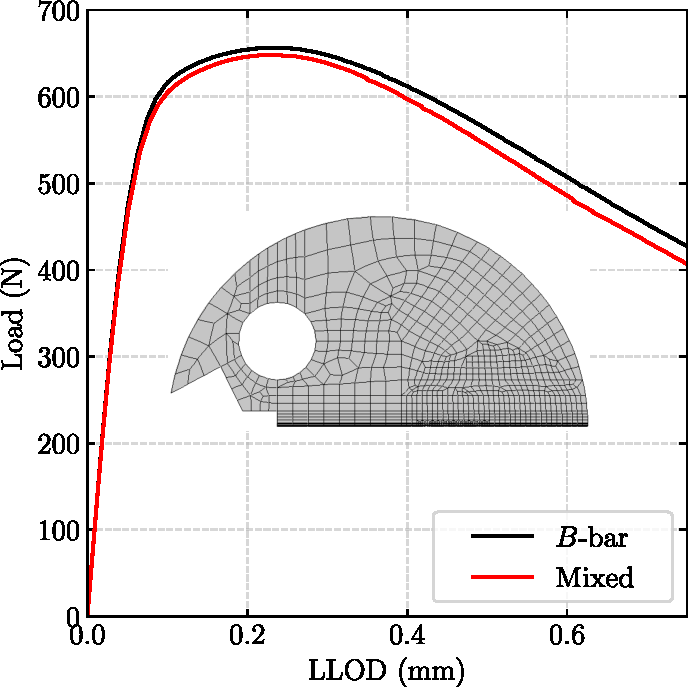
\includegraphics[width=0.7\textwidth]{Images/Load_LLOD_Bbar.pdf}
    \end{figure} 
	\end{column}
	
	\begin{column}{0.5\textwidth}
		\begin{figure}
        \centering
        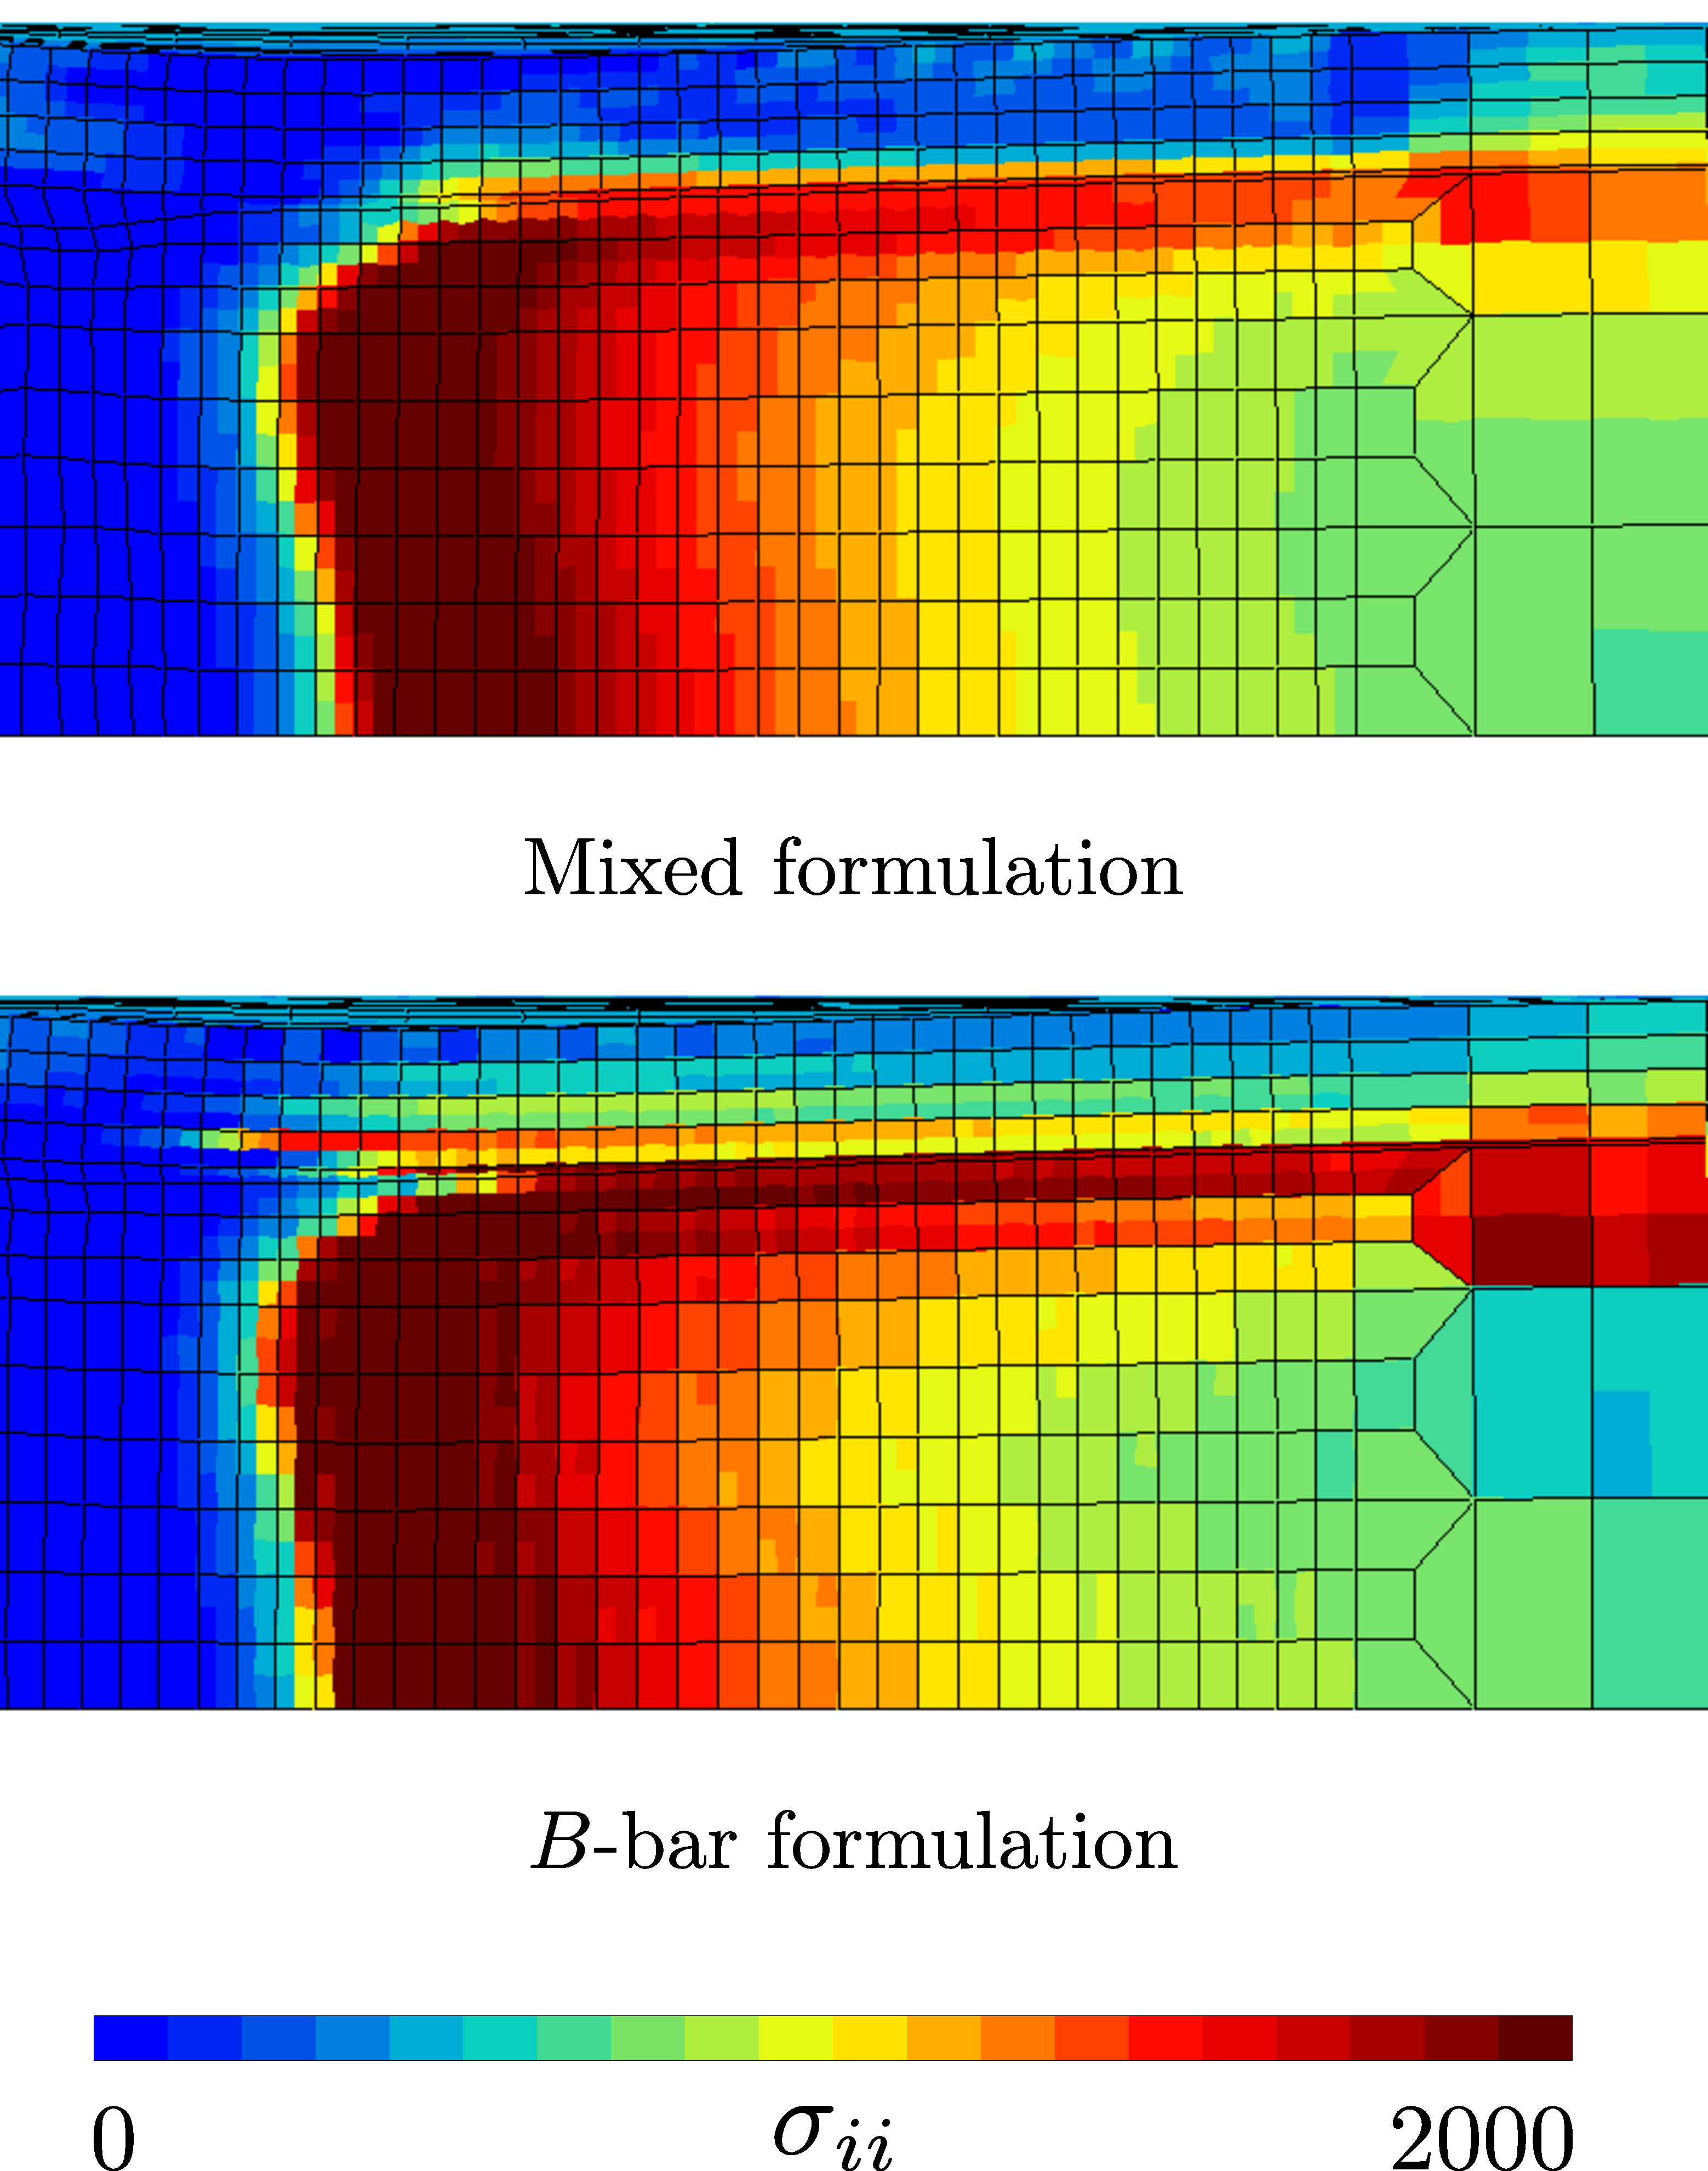
\includegraphics[width=0.6\textwidth]{Images/pressure_Bbar.pdf}
    \end{figure} 
	\end{column}
\end{columns}

\end{frame}

%%%%%%%%%%%%%%%%%%%%%%%%%%%%%%%%%%%%%%%%%%%%%%%%%%%%%%%%%%%

\begin{frame}{Nonlocal damage model}

\begin{itemize}
	\item Damage models such as the GTN model are known to induce \textbf{spurious mesh dependency} (element size, type and orientation)
	\vspace{0.25cm}
	\item To solve this problem, it is proposed to use a \textbf{nonlocal damage model} based on the \textbf{implicit gradient} by \textcolor{darkgray}{Peerlings \textit{et al.}, 1996}
\end{itemize}

	\vspace{0.25cm}

	\begin{figure}
        \centering
        \includegraphics[width=0.9\textwidth]{Images/mesh_dependency.pdf}
    \end{figure} 
    
    \begin{textblock}{5}(7.2,14.25)
        \textcolor{darkgray}{\footnotesize (Besson, 2021)}
    \end{textblock}

\end{frame}

%%%%%%%%%%%%%%%%%%%%%%%%%%%%%%%%%%%%%%%%%%%%%%%%%%%%%%%%%%%

\begin{frame}{Nonlocal damage model}

	\begin{itemize}
		\item Two variables are used (two associated internal lengths: $\bar{\omega}$ and $\bar{\kappa}$):
		
		\vspace{0.15cm}
		
        \begin{itemize}

            \item $ \displaystyle \textbf{Plastic volume variation:} \hspace{0.7cm} \textcolor{blue}{\bar{\omega}} - \ell_{\omega}^2 \Delta \textcolor{blue}{\bar{\omega}} = \omega \hspace{0.3cm} \textrm{where} \hspace{0.3cm} \omega = \textrm{trace}(\dot{\underline{\varepsilon}}_p)$
            
            \vspace{0.3cm}
            
            \item $ \displaystyle \textbf{Accumulated plastic strain:} \hspace{0.3cm} \textcolor{red}{\bar{\kappa}} - \ell_{\kappa}^2 \Delta \textcolor{red}{\bar{\kappa}} = \kappa \hspace{3.6cm}$

        \end{itemize}
        
        \vspace{0.3cm}
        
		\item The modified evolution laws for the damage variables are now:
		
        \vspace{0.3cm}
        
        \begin{itemize}
        
            \item \textbf{Void growth:} \hspace{0.7cm} $ \displaystyle \dot{f_g} = (1-f_g) \textcolor{blue}{\dot{\bar{\omega}}} $
            
            \vspace{0.3cm}
            
            \item \textbf{Void nucleation:} \hspace{0.2cm} $ \displaystyle \dot{f_n} = A_n \textcolor{red}{\dot{\bar{\kappa}}} + B_n(C) \textcolor{red}{\dot{\bar{\kappa}}}$
            
        \end{itemize}        
               
	\end{itemize}
	
	\vspace{2.65cm}
	
	\begin{tikzpicture}[remember picture, overlay]
    	\node at (current page.south west) [xshift=4.5cm, yshift=2cm] {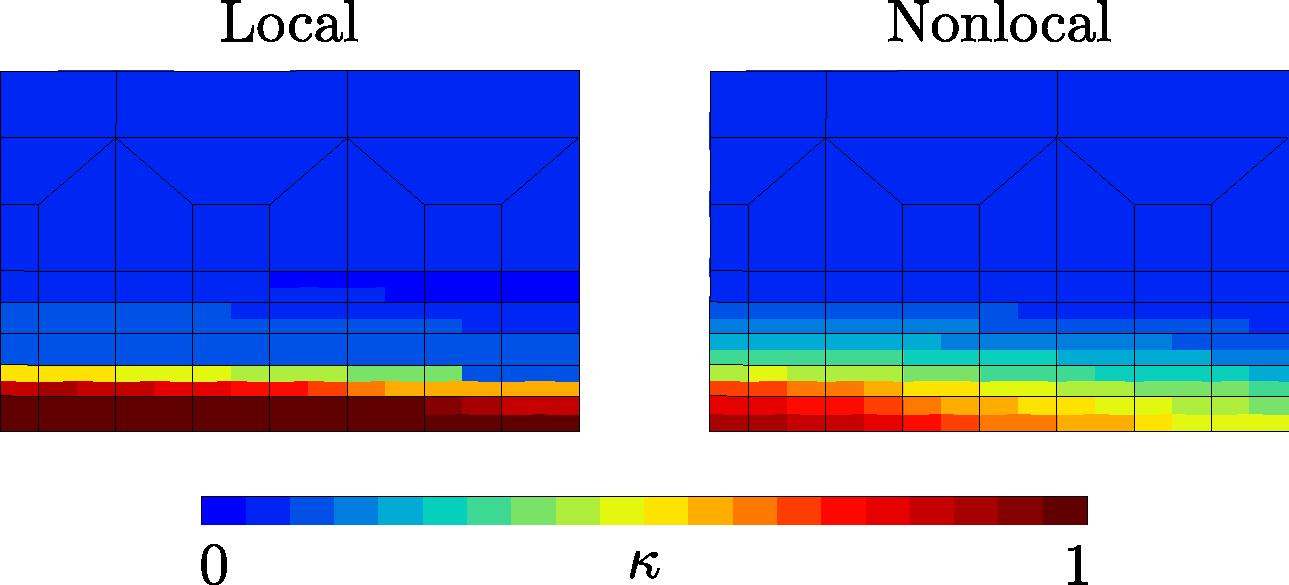
\includegraphics[width=6cm]{Images/comp_kappa.pdf}}; 
    \end{tikzpicture}
    
    \begin{tikzpicture}[remember picture, overlay]
    	\node at (current page.south west) [xshift=10.5cm, yshift=3cm] {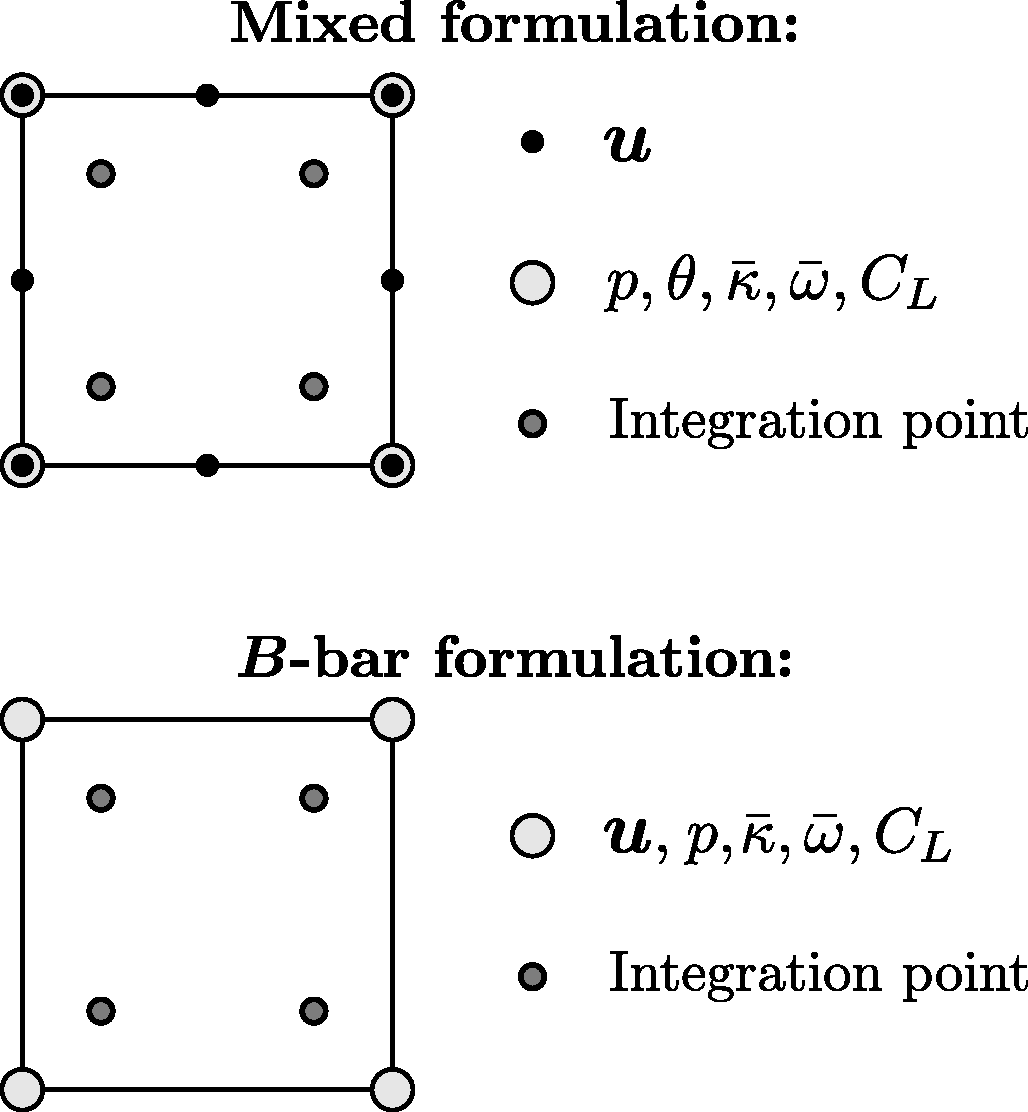
\includegraphics[width=4cm]{Images/elements.pdf}}; 
    \end{tikzpicture}

\end{frame}

%%%%%%%%%%%%%%%%%%%%%%%%%%%%%%%%%%%%%%%%%%%%%%%%%%%%%%%%%%%

\section{Numerical simulations}

\subsection{Pressurized disks tests}

\begin{frame}{Outline}
	\tableofcontents[ 
    currentsubsection, 
    hideothersubsections, 
    sectionstyle=show/shaded, 
    subsectionstyle=show/shaded, 
    ] 
\end{frame}

%%%%%%%%%%%%%%%%%%%%%%%%%%%%%%%%%%%%%%%%%%%%%%%%%%%%%%%%%%%

\begin{frame}{Context}

	\begin{itemize}
		\item \textbf{ISO 11114-4 standard:} uses pressurized disk tests for selecting metallic materials resistant to hydrogen embrittlement
		\vspace{0.15cm}
		\item Disk often fails in the clamping zone
		\vspace{0.15cm}
		\item \textbf{\textcolor{MINESBlue}{First step:}} redesigning the disk geometry to control failure location
	\end{itemize}
	
	\vspace{5cm}
	
	\begin{tikzpicture}[remember picture, overlay]
    	\node at (current page.south west) [xshift=3cm, yshift=3.5cm] {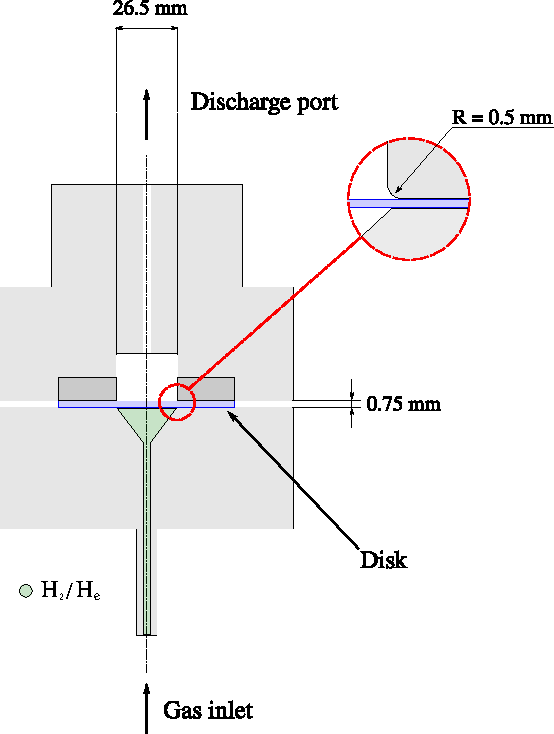
\includegraphics[width=4cm]{Images/machine_DPT.pdf}}; 
    \end{tikzpicture}
    
    \begin{tikzpicture}[remember picture, overlay]
    	\node at (current page.south west) [xshift=6.75cm, yshift=5.5cm] {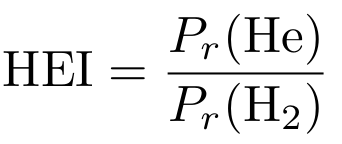
\includegraphics[width=2.cm]{Images/HEI.png}}; 
    \end{tikzpicture}
    
    \begin{tikzpicture}[remember picture, overlay]
    	\node at (current page.south west) [xshift=6.35cm, yshift=3cm] {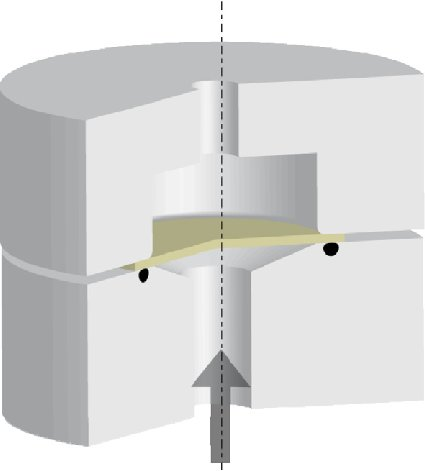
\includegraphics[width=2.75cm]{Images/machine_DPT_2.jpg}}; 
    \end{tikzpicture}
    
    \begin{tikzpicture}[remember picture, overlay]
    	\node at (current page.south west) [xshift=10.5cm, yshift=5cm] {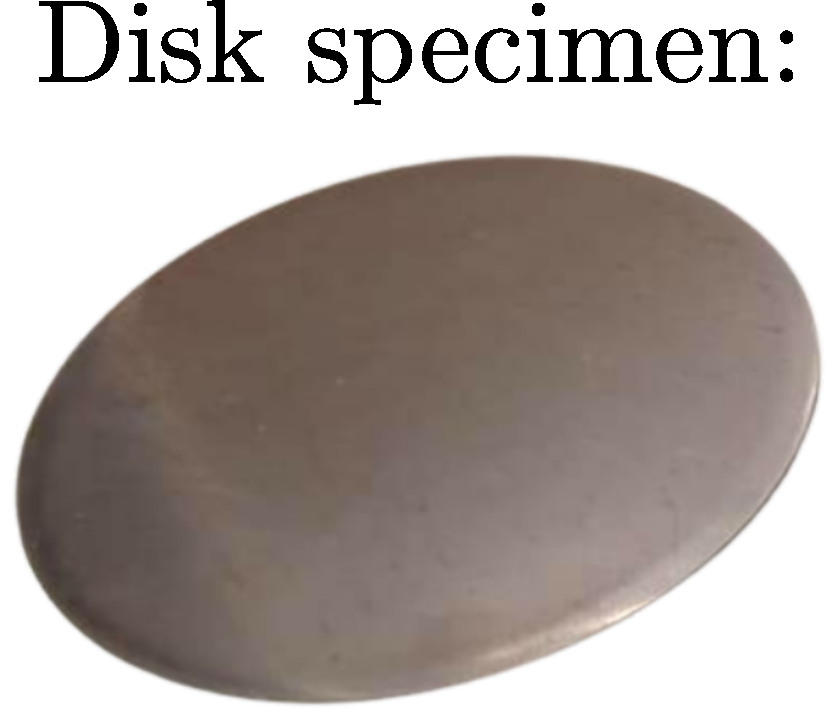
\includegraphics[width=2.cm]{Images/std_disk.pdf}}; 
    \end{tikzpicture}
    
    \begin{tikzpicture}[remember picture, overlay]
    	\node at (current page.south west) [xshift=10.5cm, yshift=2.5cm] {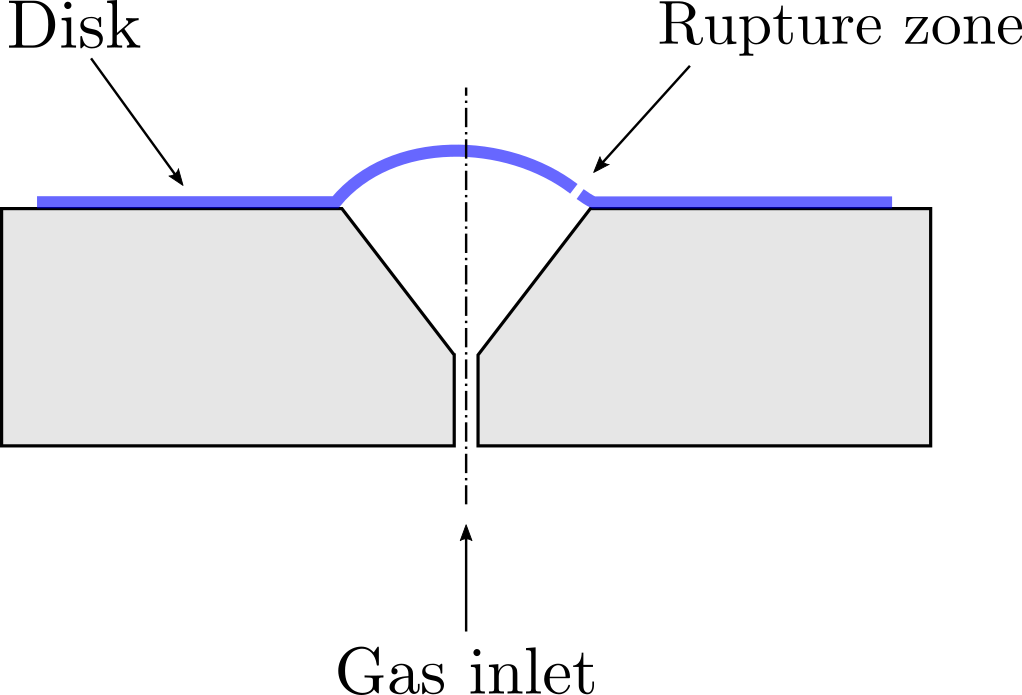
\includegraphics[width=4cm]{Images/rupture_disk.png}}; 
    \end{tikzpicture}
	
\end{frame}

%%%%%%%%%%%%%%%%%%%%%%%%%%%%%%%%%%%%%%%%%%%%%%%%%%%%%%%%%%%

\begin{frame}{Redesign of the disk geometry}

\begin{itemize}
	\item New proposed geometries:
	\vspace{0.15cm}
	\begin{itemize}
		\item No need to modify the test setup
		\vspace{0.15cm}
		\item Keep the same minimum thickness of the standard (0.75 mm)
		\vspace{0.15cm}
	\end{itemize}
	\item Optimization with respect to $\ell$, $R$ and $R^\prime$ with FE simulations considering an elasto-plastic behavior
\end{itemize}

\begin{figure}
	\centering
	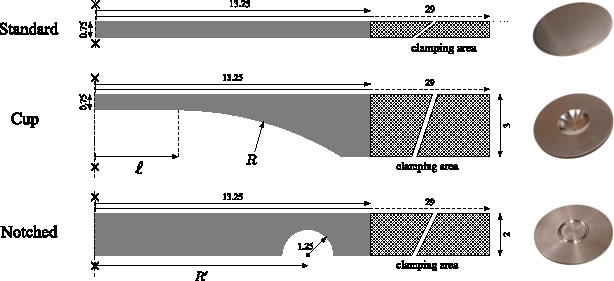
\includegraphics[width=0.9\textwidth]{Images/disks.pdf}
\end{figure}

\end{frame}

%%%%%%%%%%%%%%%%%%%%%%%%%%%%%%%%%%%%%%%%%%%%%%%%%%%%%%%%%%%

\begin{frame}{Redesign of the disk geometry}

\begin{itemize}
	\item The location of the maximum accumulated plastic strain ($\kappa$) corresponds to the failure location
\end{itemize}

\vspace{0.5cm}

\begin{figure}
	\centering
	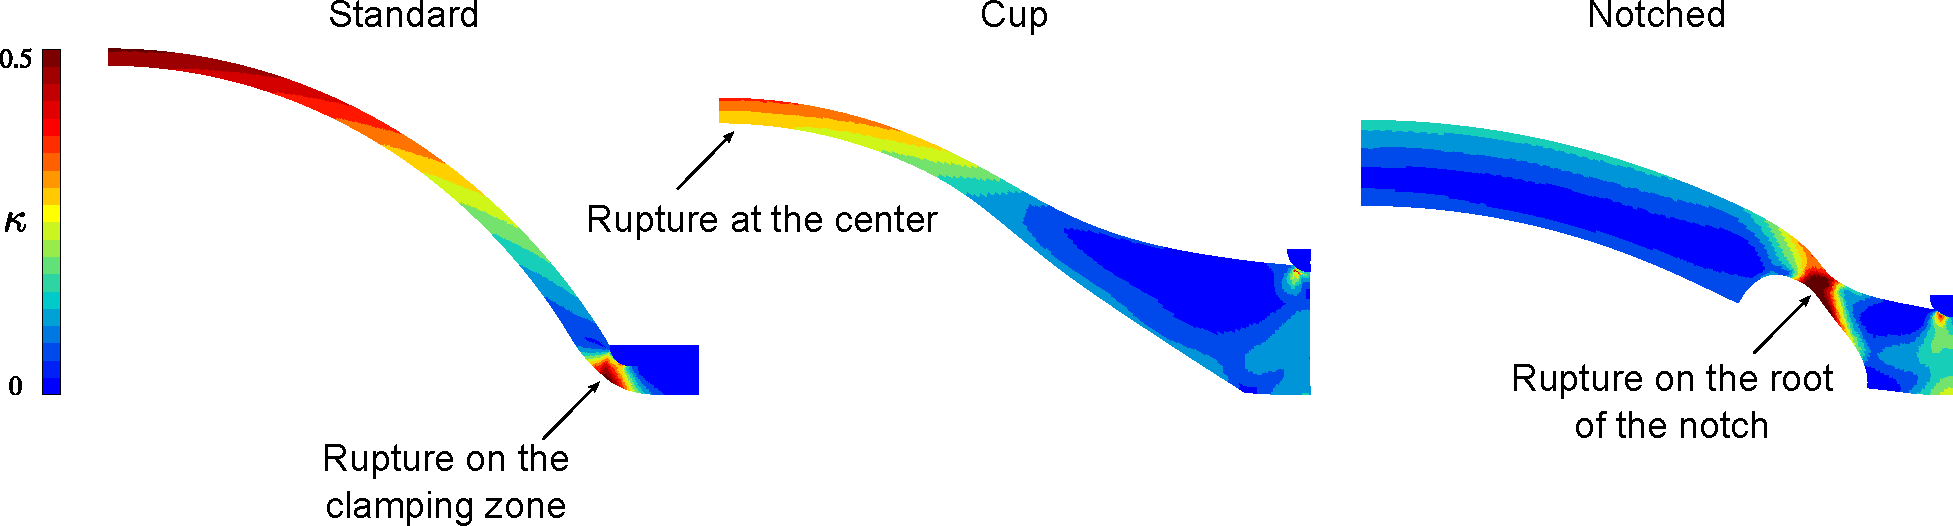
\includegraphics[width=0.95\textwidth]{Images/disks_rupture.pdf}
\end{figure}

\end{frame}

%%%%%%%%%%%%%%%%%%%%%%%%%%%%%%%%%%%%%%%%%%%%%%%%%%%%%%%%%%%

\begin{frame}{Materials}

\begin{columns}
\begin{column}{0.65\textwidth}

\begin{itemize}
	\item \textbf{X52 vintage steel:}
	\vspace{0.3cm}
	\begin{itemize}
		\item Yield strength: 400 MPa
		\vspace{0.3cm}
		\item Different elongation at rupture in T and L directions
	\end{itemize}
	
	\vspace{0.35cm}
	
	\item \textbf{E355 mod. steel:}
	
	\vspace{0.3cm}
	
	\begin{itemize}
		\item Yield strength: 330 MPa
		\vspace{0.3cm}
		\item Higher elongation at rupture and lower Ultimate Tensile Strength in relation with the vintage material
		\vspace{0.cm}
		\item Similar elongation at rupture in both directions
	\end{itemize}
	
	\vspace{0.35cm}	
	
	\item Elasto(visco)-plastic model coefficients' identified through optimization: \\
	
	\begin{figure}
	\centering
	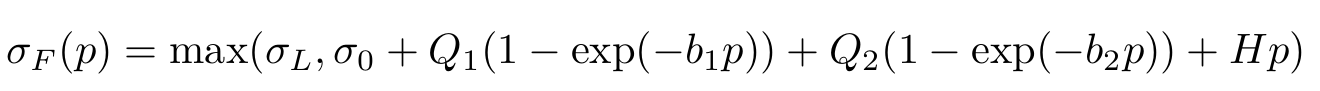
\includegraphics[width=0.98\textwidth]{Images/voce_law.png} \\
\end{figure}

\end{itemize}

\end{column}

\begin{column}{0.35\textwidth}
	
\begin{figure}
	\centering
	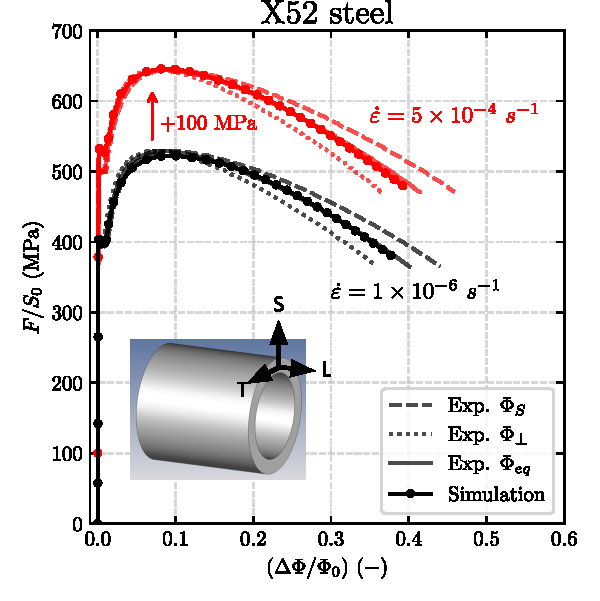
\includegraphics[width=0.95\textwidth]{Images/plot_X52_radial.pdf} \\
	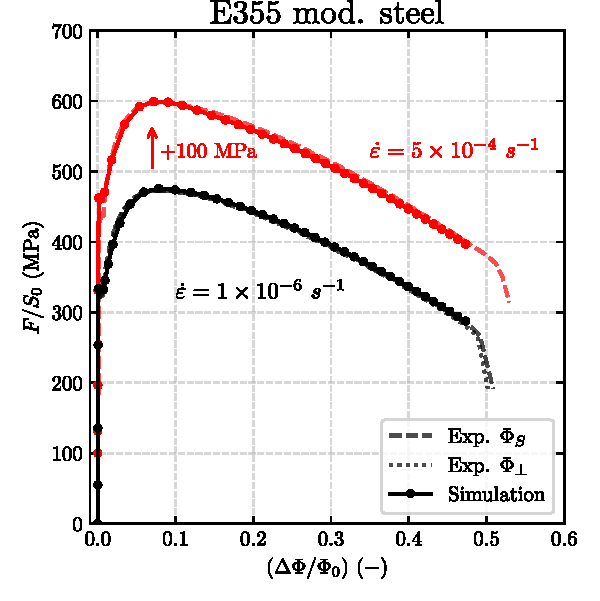
\includegraphics[width=0.95\textwidth]{Images/plot_E355_radial.pdf}
\end{figure}

\end{column}

\end{columns}

\end{frame}

%%%%%%%%%%%%%%%%%%%%%%%%%%%%%%%%%%%%%%%%%%%%%%%%%%%%%%%%%%%

\begin{frame}{Simulation of pressurized disks}

\begin{itemize}
	\item Axisymmetric model, quadratic elements with reduced integration (mixed formulation)
	\vspace{0.15cm}
	\item Hydrogen diffusion parameters taken from the literature
	\vspace{0.15cm}
	\item Since damage is not considered into the numerical model, the simulations were stopped once they reached experimentally observed rupture pressure $(P_r)$
	\vspace{0.15cm} 
	\item Model's boundary conditions:
\end{itemize}

\begin{figure}
	\centering
	\includegraphics[width=0.7\textwidth]{Images/all_BC_std.pdf} \\
\end{figure}

\end{frame}

%%%%%%%%%%%%%%%%%%%%%%%%%%%%%%%%%%%%%%%%%%%%%%%%%%%%%%%%%%%

\begin{frame}{Results under helium}

\begin{itemize}
	\item Successfully modification of fracture location
	\vspace{0.15cm}
	\item Failure is primarily driven by plasticity and occurs \\ under a limit load scenario
\end{itemize}

\vspace{0.15cm}

\begin{figure}
	\centering
	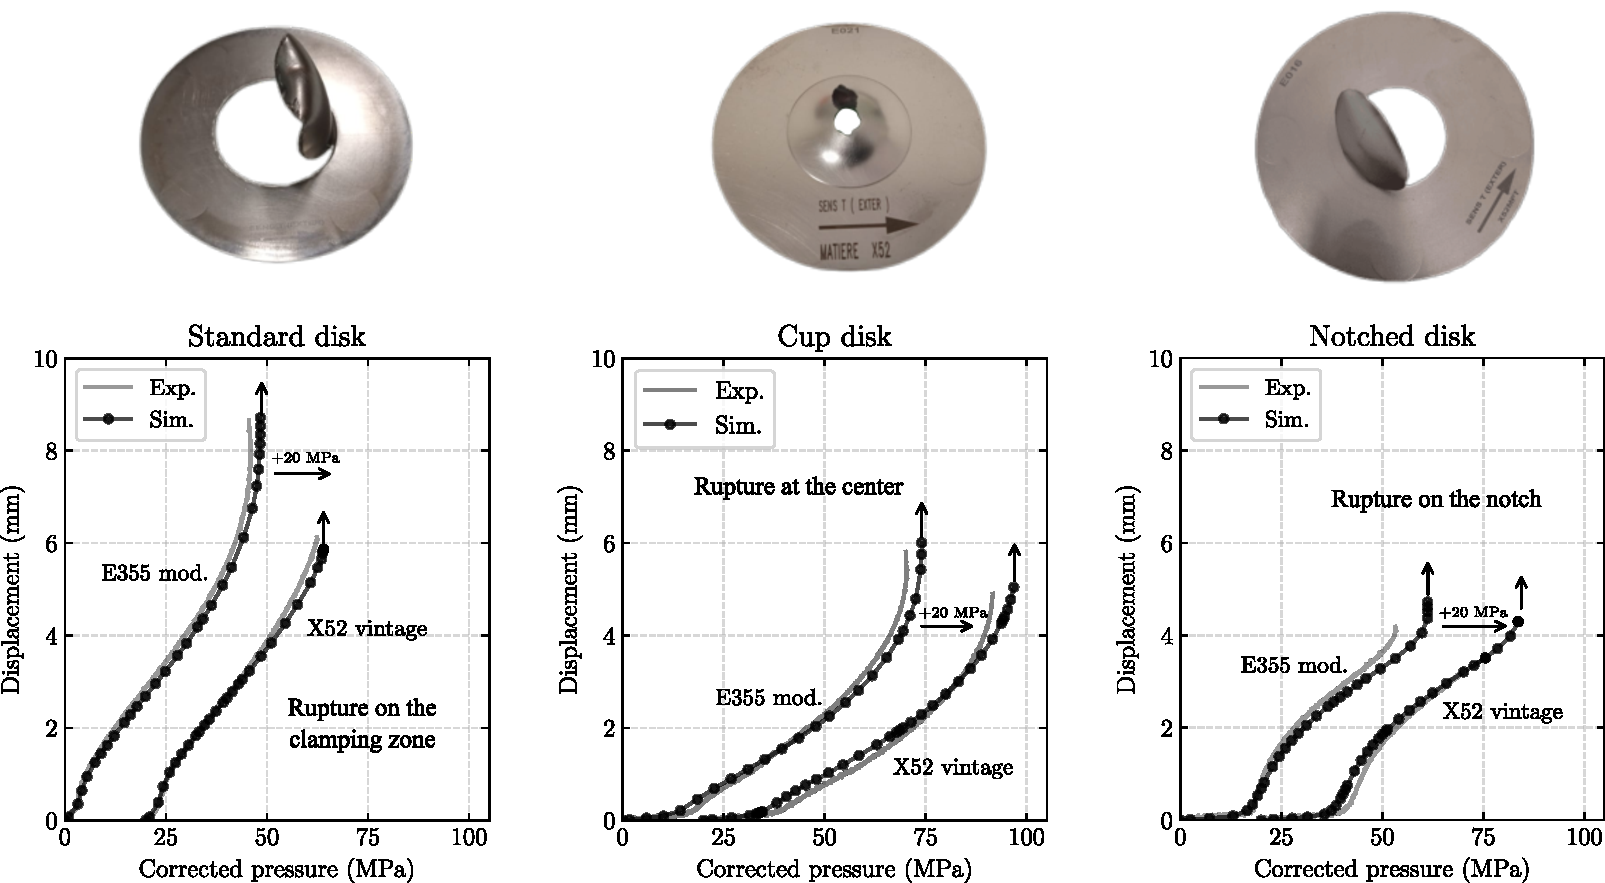
\includegraphics[width=0.85\textwidth]{Images/disks_helium.pdf} \\
\end{figure}

\begin{tikzpicture}[remember picture, overlay]
    	\node at (current page.south west) [xshift=10.2cm, yshift=7.5cm] {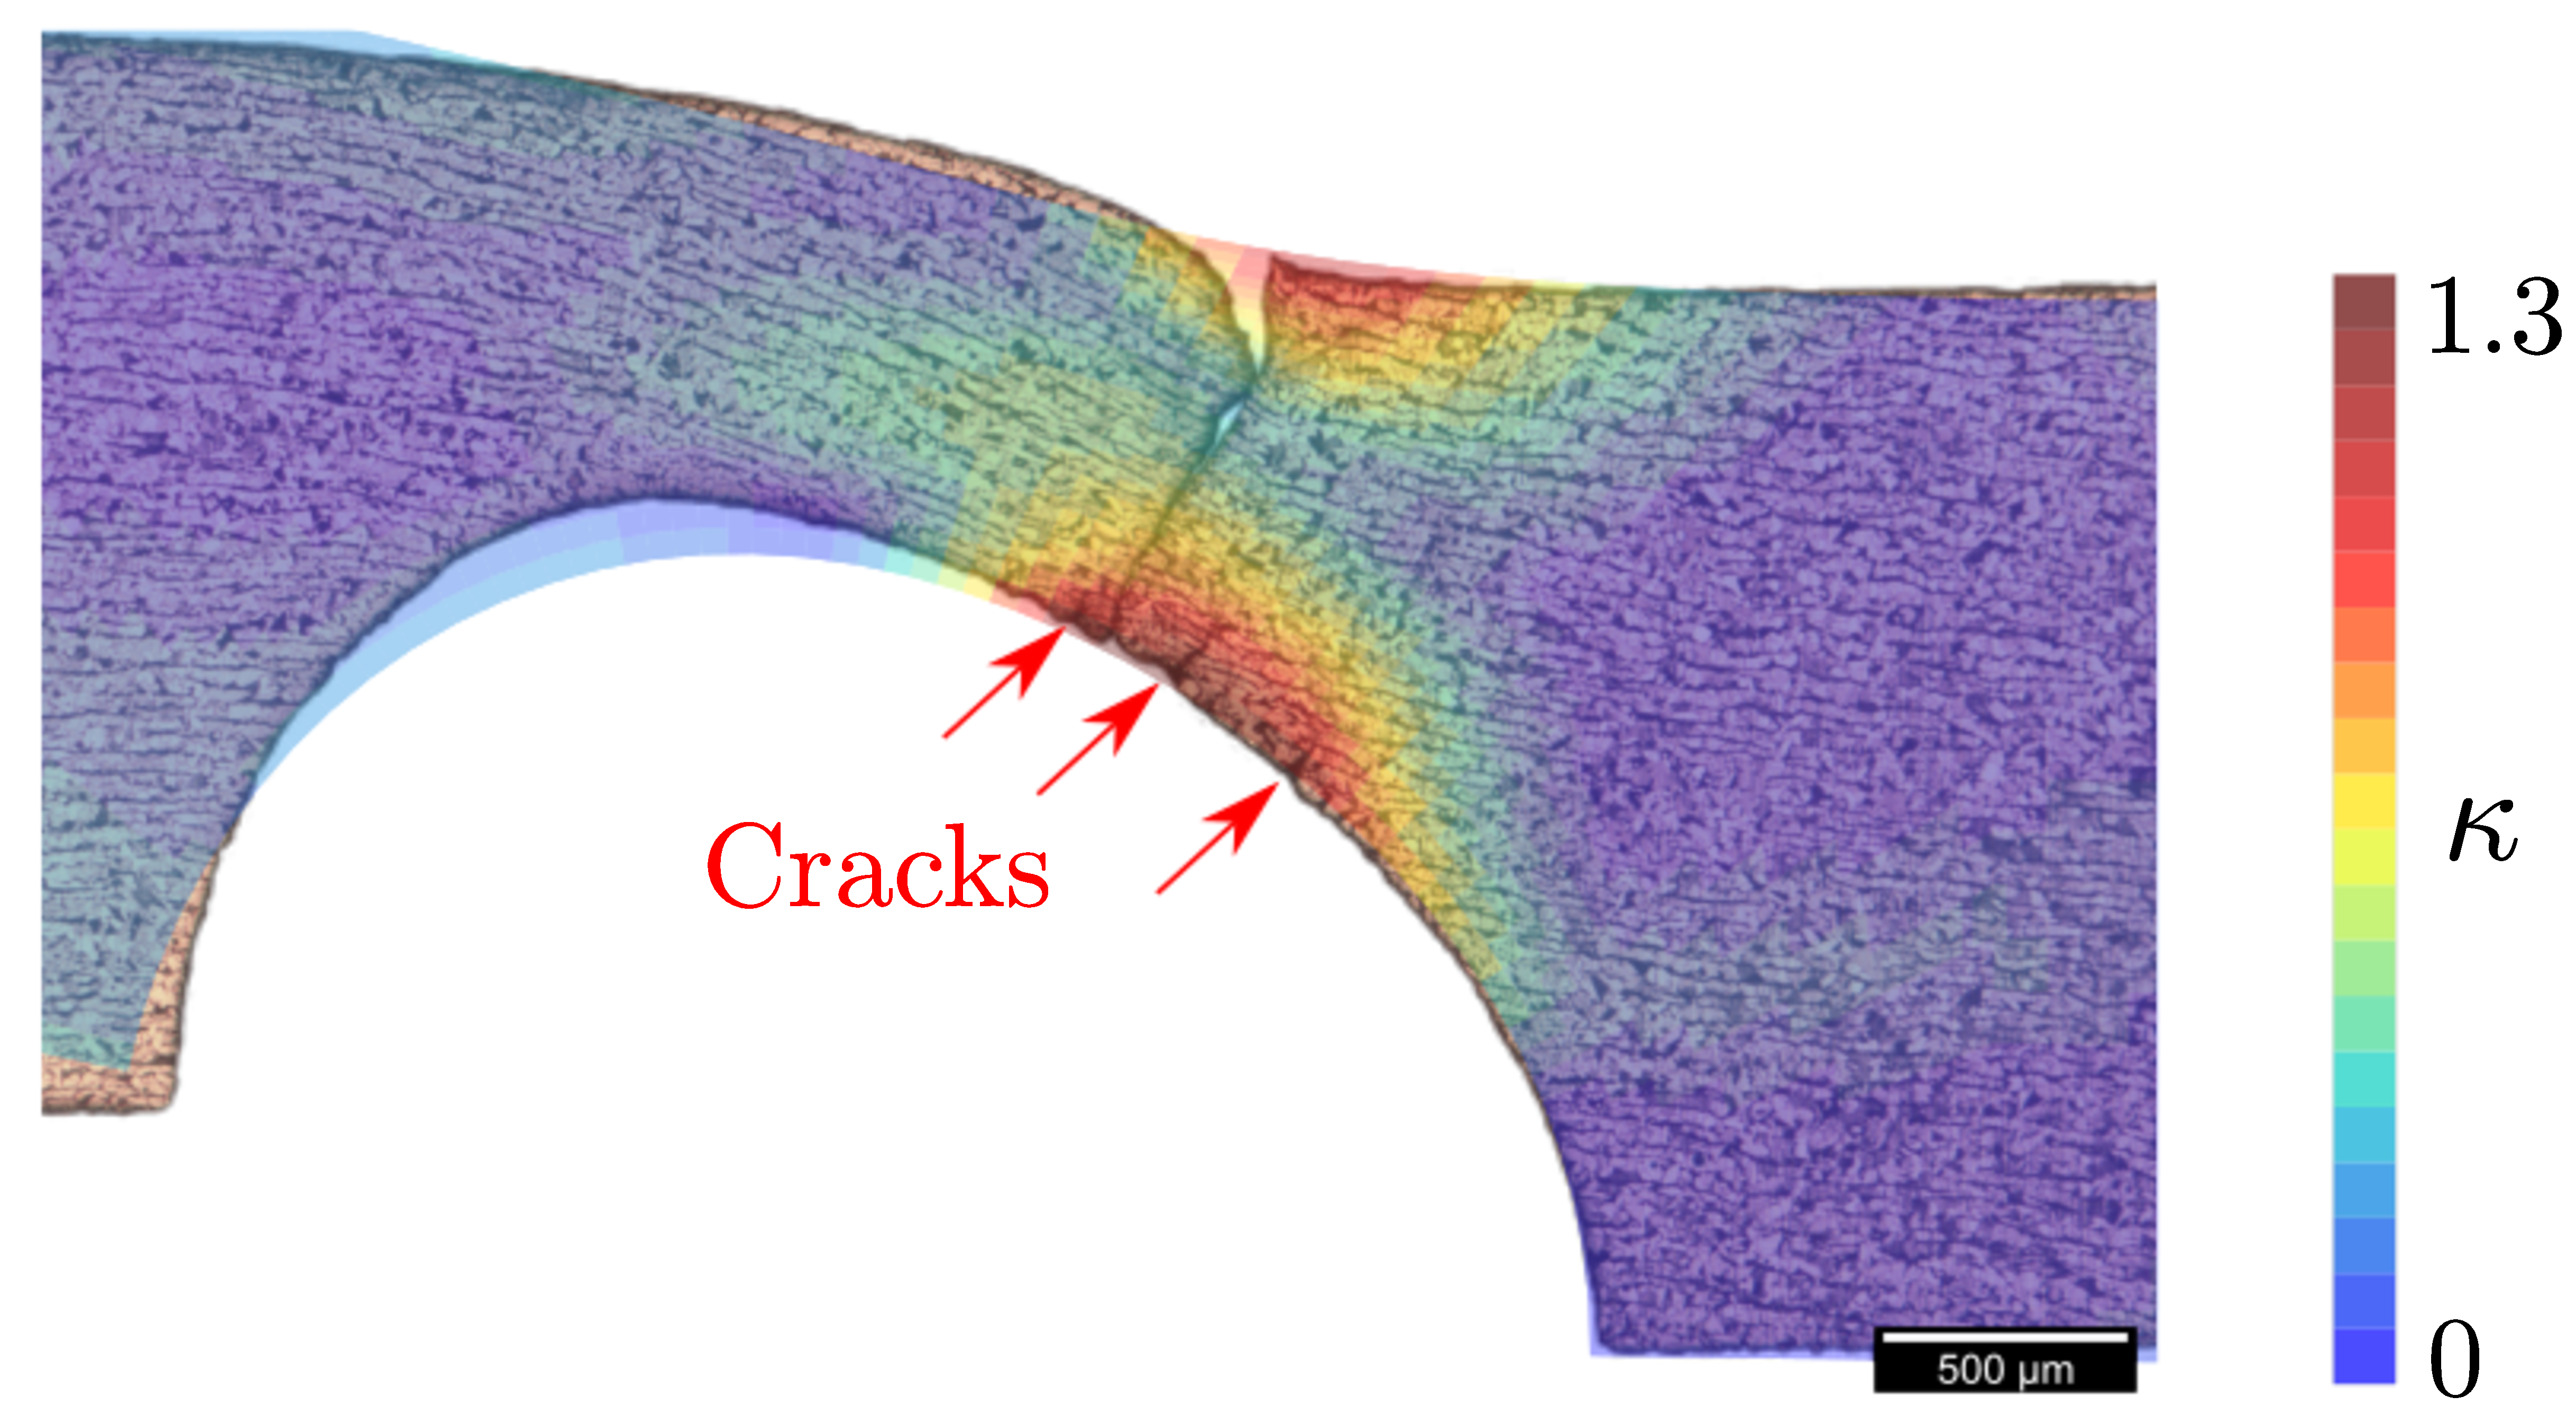
\includegraphics[width=3.75cm]{Images/fracto+simulation.png}}; 
    \end{tikzpicture}
    
    \begin{textblock}{6}(5.75,14.75)
        \textcolor{gray}{\scriptsize (Experimental data: Santana \textit{et al., 2024)}}
    \end{textblock}

\end{frame}

%%%%%%%%%%%%%%%%%%%%%%%%%%%%%%%%%%%%%%%%%%%%%%%%%%%%%%%%%%%

\begin{frame}{Results under hydrogen (E355 mod. steel)}

\begin{figure}
	\centering
	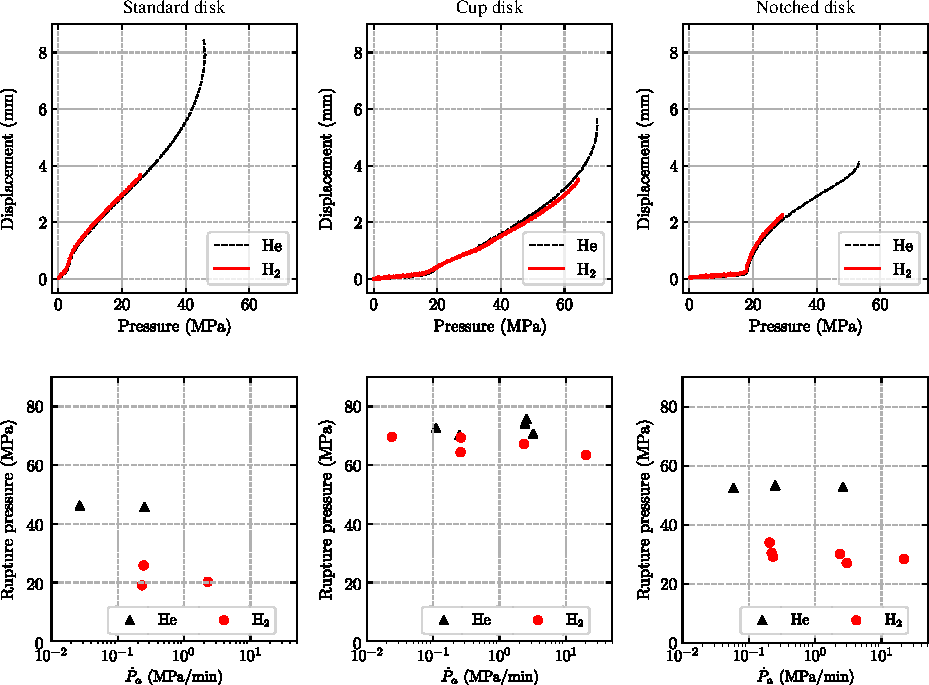
\includegraphics[width=0.85\textwidth]{Images/H2_results_E355.pdf} \\
\end{figure}

    \begin{textblock}{6}(5.75,14.9)
        \textcolor{gray}{\scriptsize (Experimental data: Santana \textit{et al., 2024)}}
    \end{textblock}

\end{frame}

%%%%%%%%%%%%%%%%%%%%%%%%%%%%%%%%%%%%%%%%%%%%%%%%%%%%%%%%%%%

\begin{frame}{Hydrogen embrittled depth}

\begin{figure}
	\centering
	\includegraphics[width=0.9\textwidth]{Images/embrittled_depth.pdf} \\
\end{figure}

    \begin{textblock}{6}(5.75,14.95)
        \textcolor{gray}{\scriptsize (Experimental data: Santana \textit{et al., 2024)}}
    \end{textblock}

\end{frame}

%%%%%%%%%%%%%%%%%%%%%%%%%%%%%%%%%%%%%%%%%%%%%%%%%%%%%%%%%%%

\begin{frame}{Hydrogen trapping model}

\begin{itemize}
	\item Considers only one kind of trap: dislocations
	\vspace{0.1cm}
	\item Trap binding energies ($W_B$) and trap densities ($N_T$) were taken from the literature and analyzed based on the experimental observations
	\vspace{0.1cm}
	\item Based on the models proposed by \textcolor{darkgray}{Moro \textit{et al.} (2010)} and \textcolor{darkgray}{Kumnick \textit{et al.} (1980)}, four cases emerge
\end{itemize}

\begin{columns}
	\begin{column}{0.55\textwidth}
	\begin{figure}
		\centering
		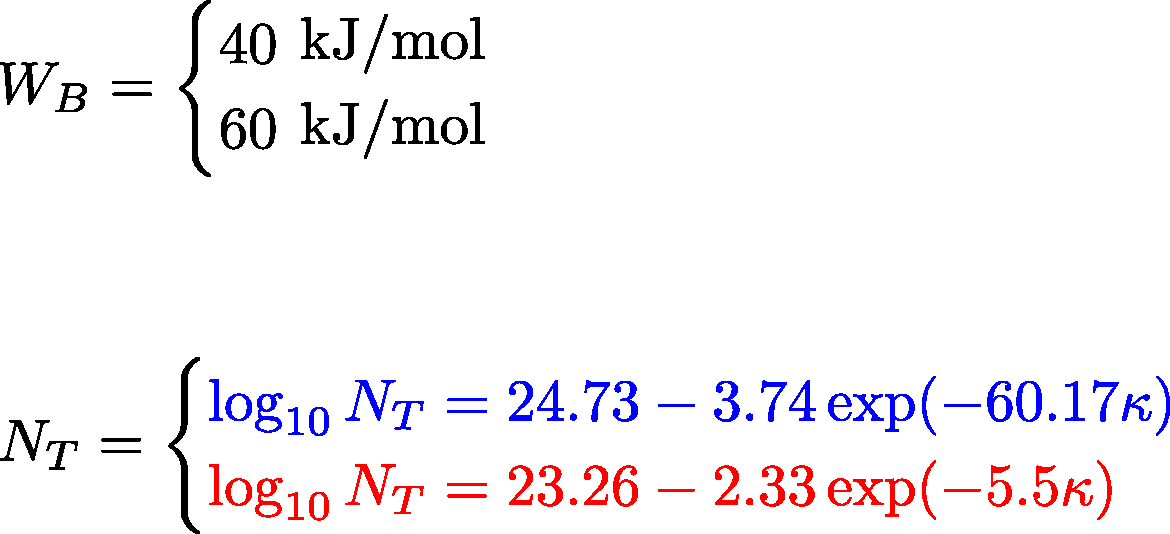
\includegraphics[width=0.95\textwidth]{Images/cases.pdf} \\
	\end{figure}
	\end{column}
	
	\begin{column}{0.45\textwidth}
	\begin{figure}
		\centering
		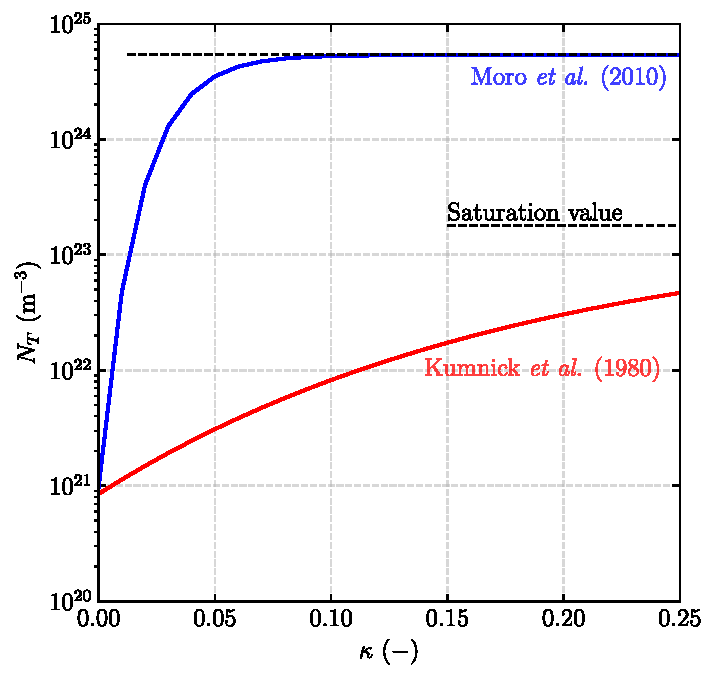
\includegraphics[width=1.0\textwidth]{Images/plot_NT_epcum.pdf} \\
	\end{figure}
	\end{column}
\end{columns}

\end{frame}

%%%%%%%%%%%%%%%%%%%%%%%%%%%%%%%%%%%%%%%%%%%%%%%%%%%%%%%%%%%

\begin{frame}{Hydrogen embrittled depth}

\begin{figure}
	\centering
	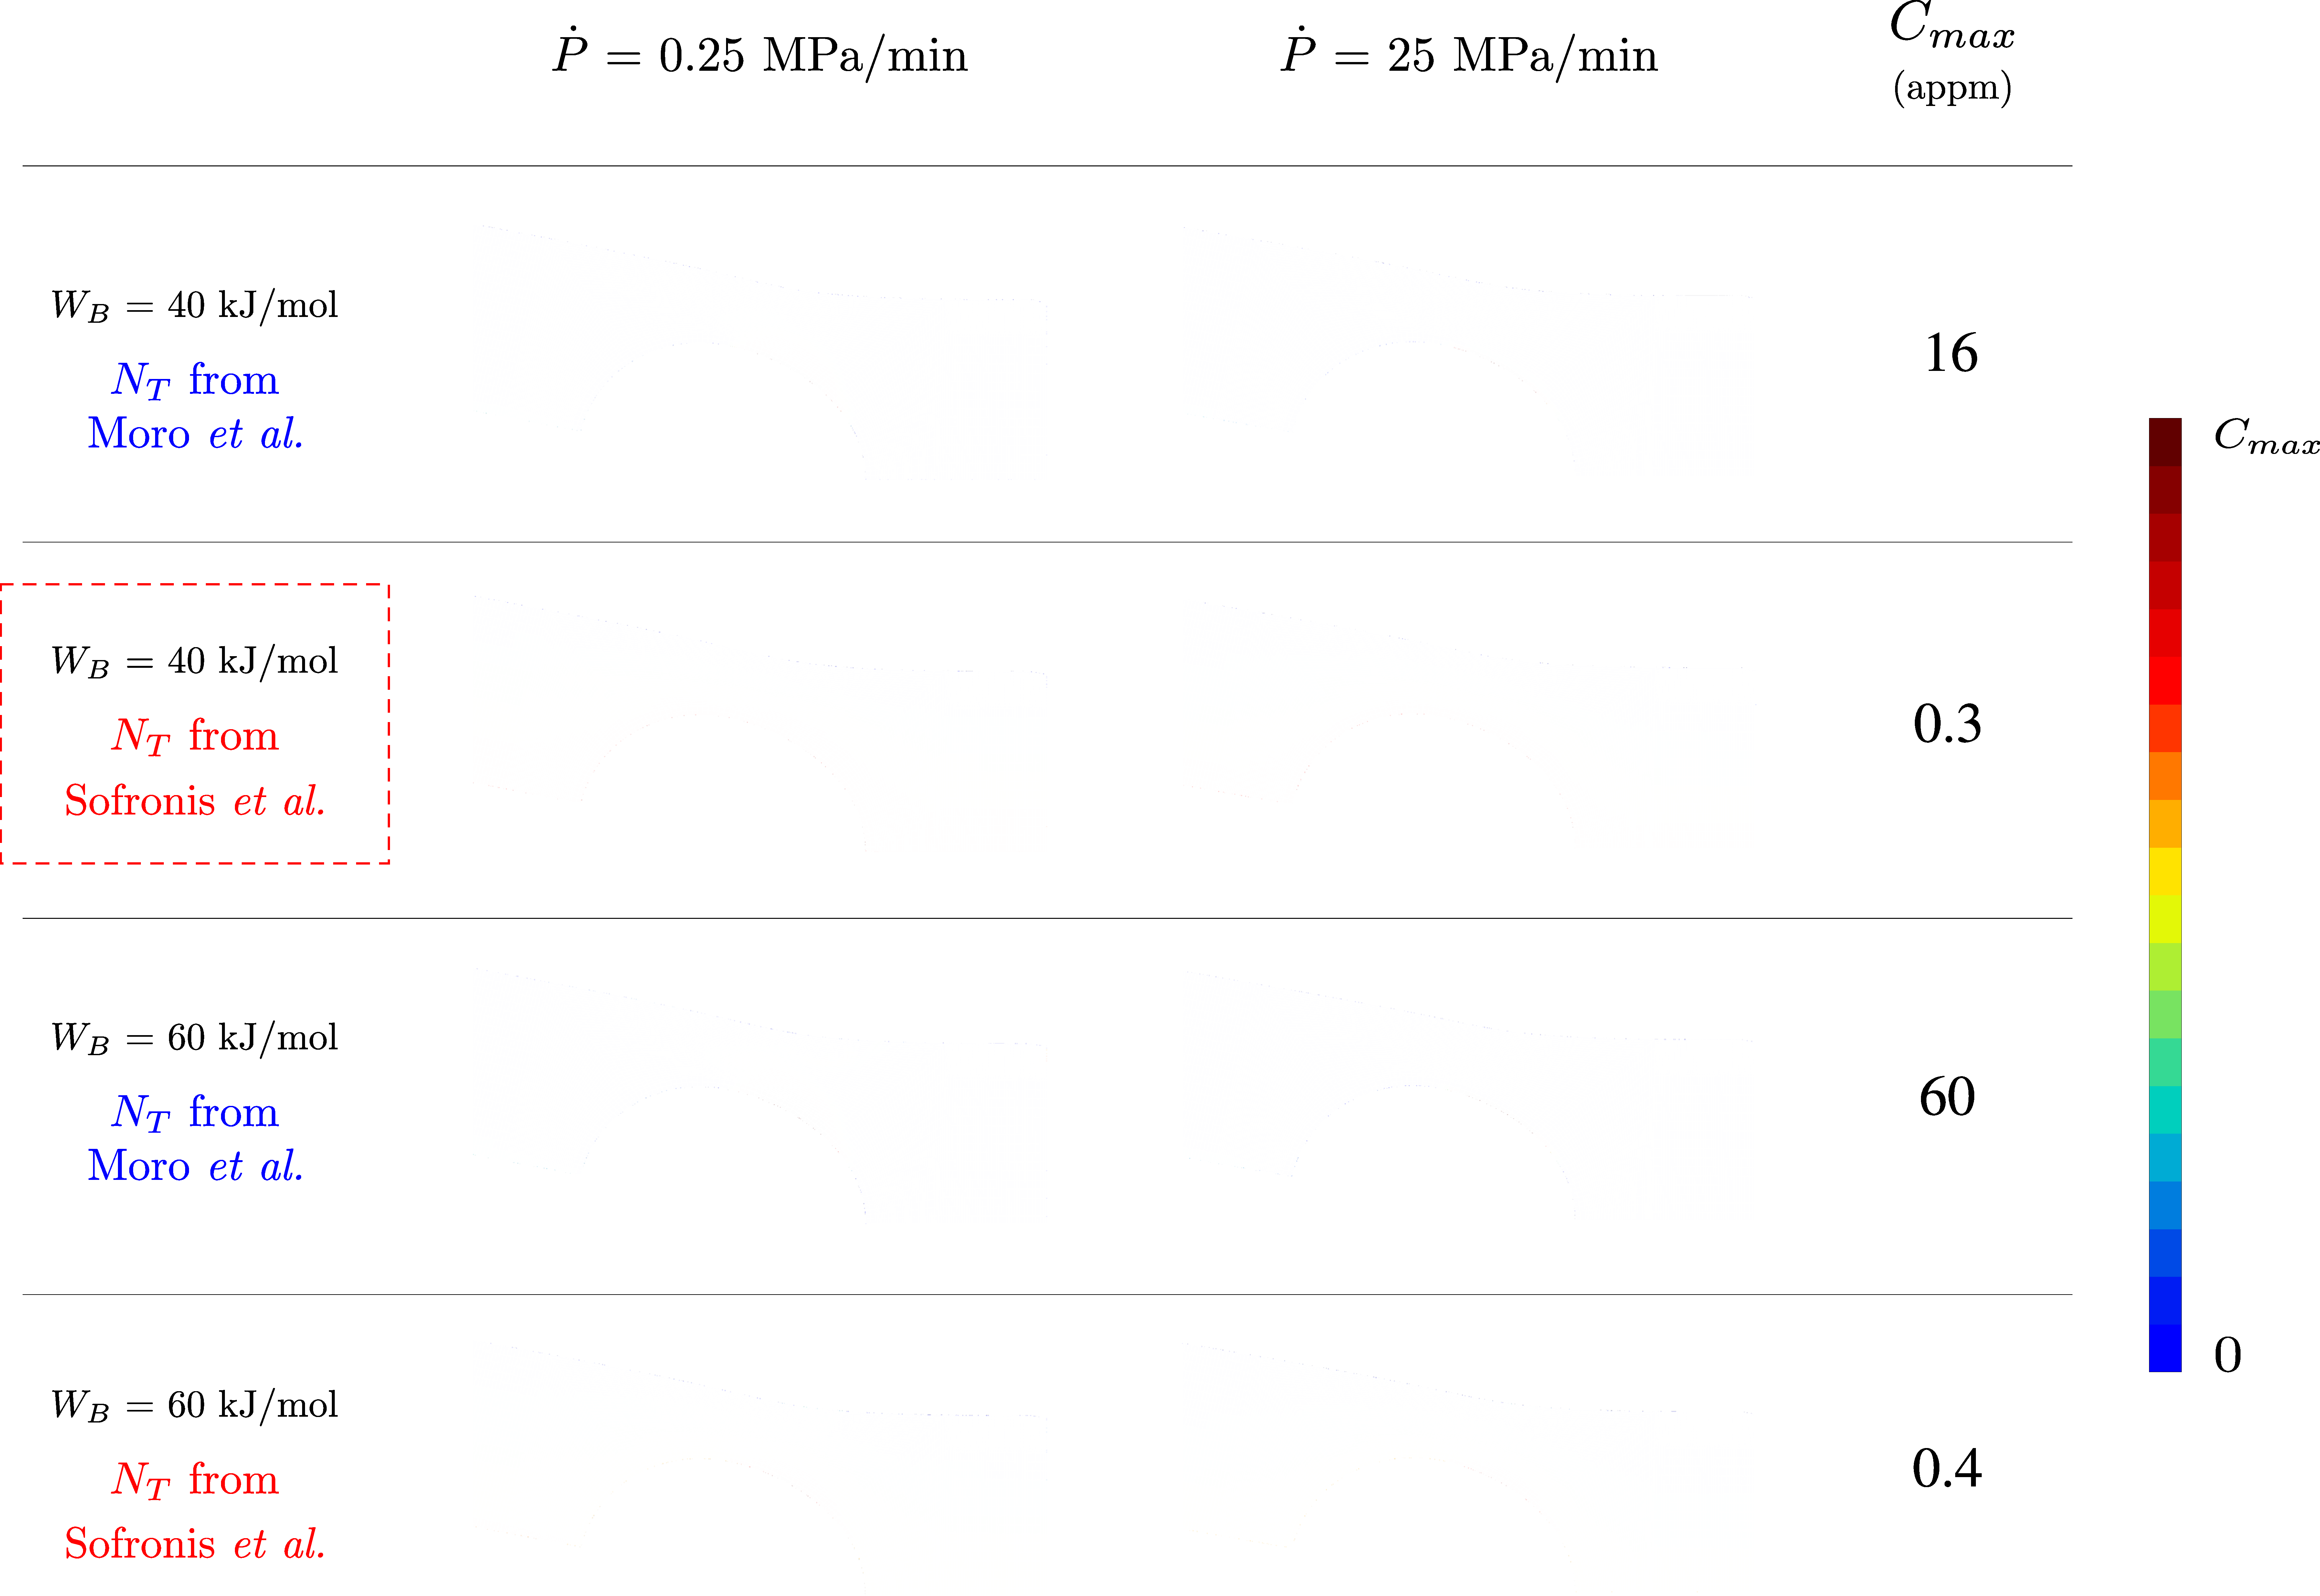
\includegraphics[width=0.9\textwidth]{Images/table_zoom.pdf} \\
\end{figure}

\end{frame}

%%%%%%%%%%%%%%%%%%%%%%%%%%%%%%%%%%%%%%%%%%%%%%%%%%%%%%%%%%%

\begin{frame}{Principal stress evolution}

\begin{itemize}
	\item Specimens that develop higher principal stress ($\sigma_I$) in the fracture zone fail at a lower hydrogen pressure ($P_a(H_2)$)
	\vspace{0.25cm}
	\item The total hydrogen concentration reduces the maximum principal stress that that triggers fracture
\end{itemize}

\begin{columns}

\begin{column}{0.49\textwidth}
	\begin{figure}
		\centering
		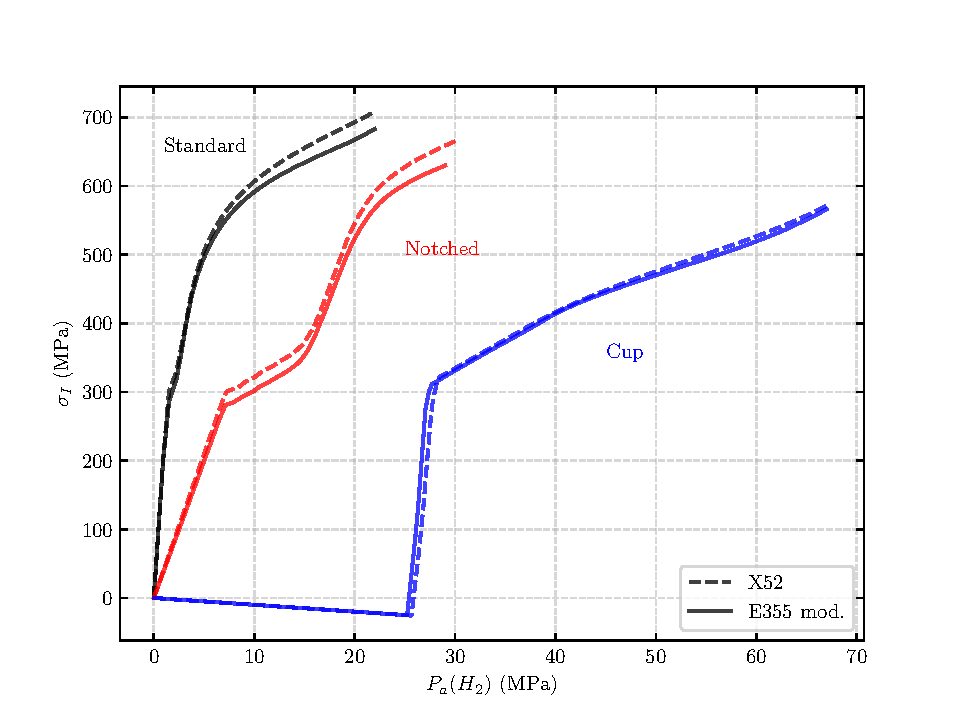
\includegraphics[width=\textwidth]{Images/sigp1_pressure.pdf} \\
	\end{figure}
\end{column}

\begin{column}{0.49\textwidth}
	\begin{figure}
		\centering
		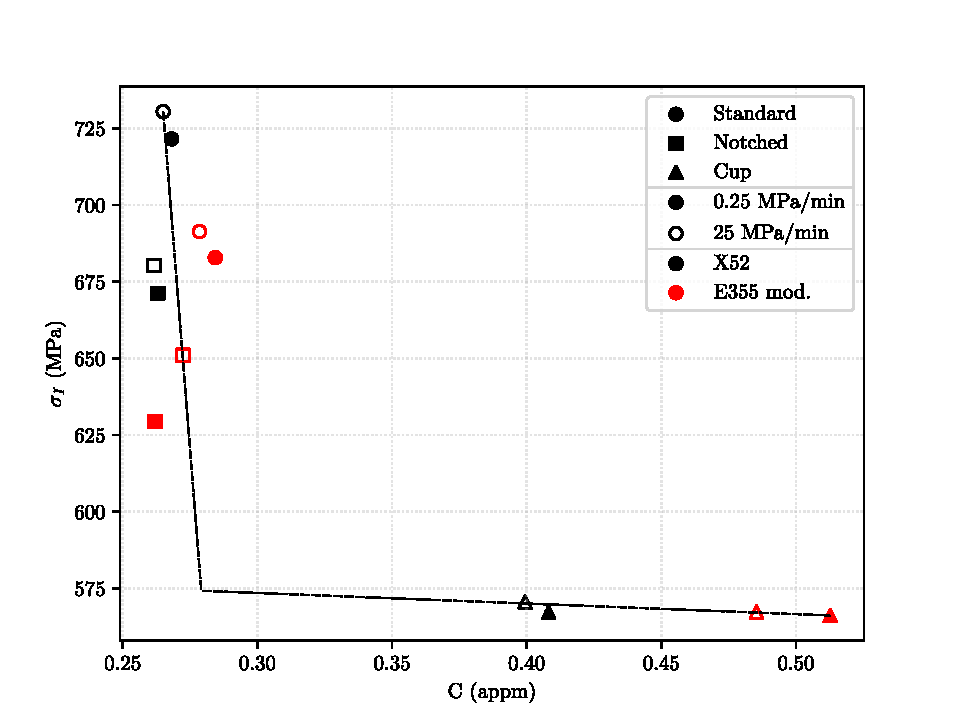
\includegraphics[width=\textwidth]{Images/plot_sigp1_C_edit.pdf} \\
	\end{figure}
\end{column}

\end{columns}

\end{frame}

%%%%%%%%%%%%%%%%%%%%%%%%%%%%%%%%%%%%%%%%%%%%%%%%%%%%%%%%%%%

%\subsection{Hydrogen uptake during a tensile test}
%
%\begin{frame}{Outline}
%	\tableofcontents[ 
%    currentsubsection, 
%    hideothersubsections, 
%    sectionstyle=show/shaded, 
%    subsectionstyle=show/shaded, 
%    ] 
%\end{frame}
%
%%%%%%%%%%%%%%%%%%%%%%%%%%%%%%%%%%%%%%%%%%%%%%%%%%%%%%%%%%%%
%
%\begin{frame}{Experimental procedure}
%
%\textbf{\textcolor{MINESBlue}{\large Tensile test:}}
%\vspace{0.1cm}
%\begin{itemize}
%	\item Material: X52 vintage steel
%	\vspace{0.1cm}
%	\item Gaseous atmosphere under different conditions:
%\vspace{0.1cm}
%\begin{table}[ht!]
%	\small
%    \centering
%    \renewcommand{\arraystretch}{1.5}
%    \begin{tabular}{ll}
%    \textbf{Environment}                 & Air, 85 bar H$_\text{2}$                               \\ \hline
%    \textbf{Strain}                 & 0\%, 30\%Rp02, 90\%Rp02, 3\%, 6\%, 12\%             \\ \hline
%    \textbf{Strain Rate (s$^{-1}$)} & $1\times10^{-5}$, $1\times10^{-4}$, $1\times10^{-3}$ \\ \hline
%    \textbf{Dwell}                       & No dwell, Dwell                                     
%    \end{tabular}
%\end{table}
%	
%\end{itemize}
%
%\begin{columns}
%
%\begin{column}{0.49\textwidth}
%	\begin{figure}
%		\centering
%		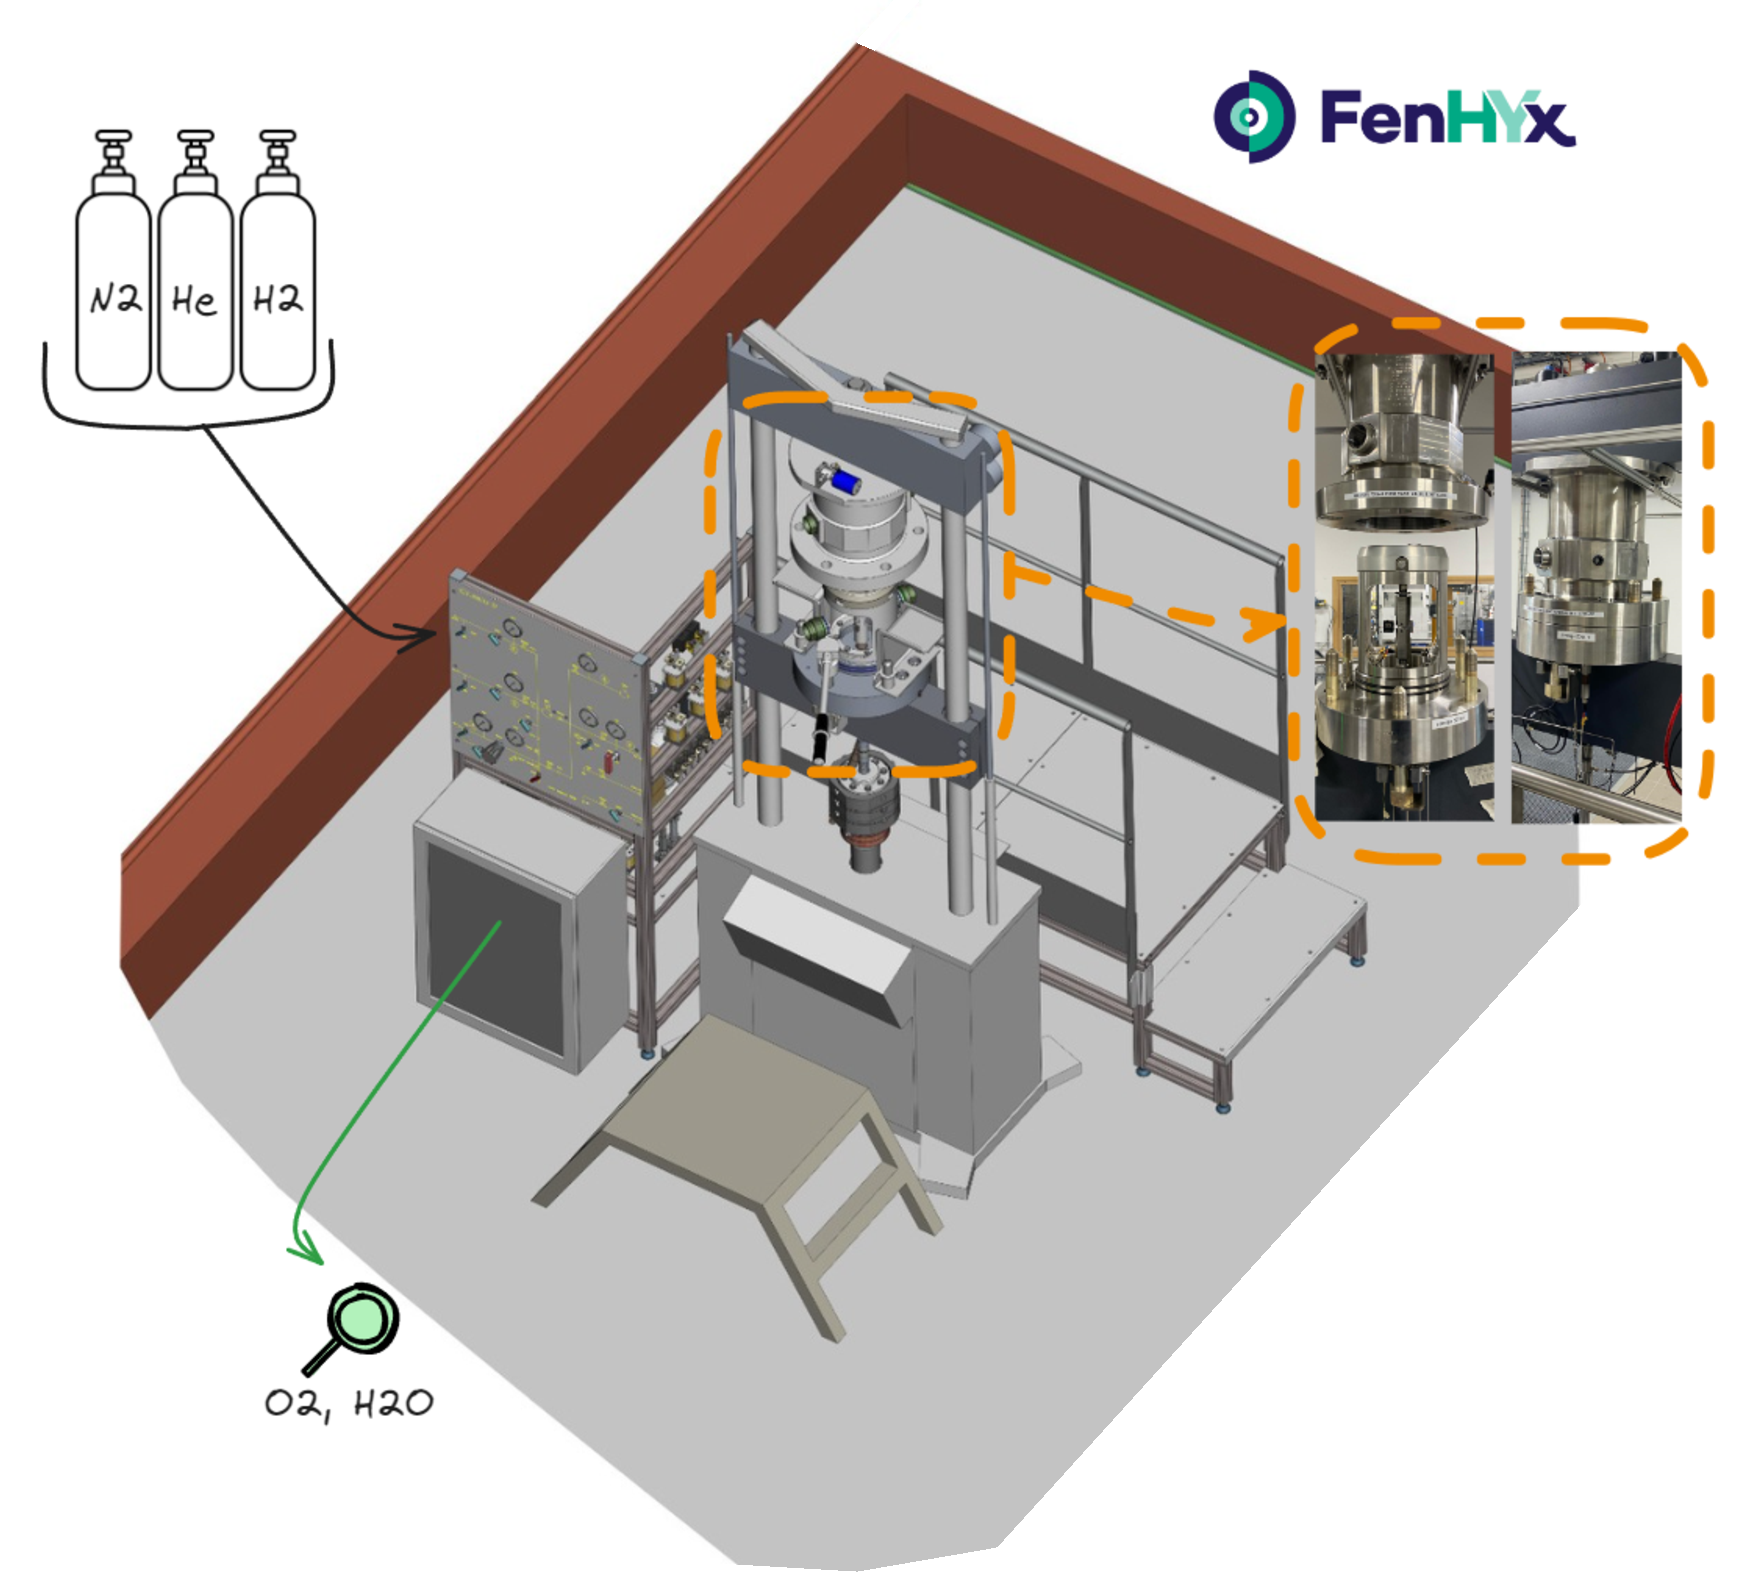
\includegraphics[width=0.8\textwidth]{Images/machine_fenhyx.pdf} \\
%	\end{figure}
%\end{column}
%
%\begin{column}{0.49\textwidth}
%	\begin{figure}
%		\centering
%		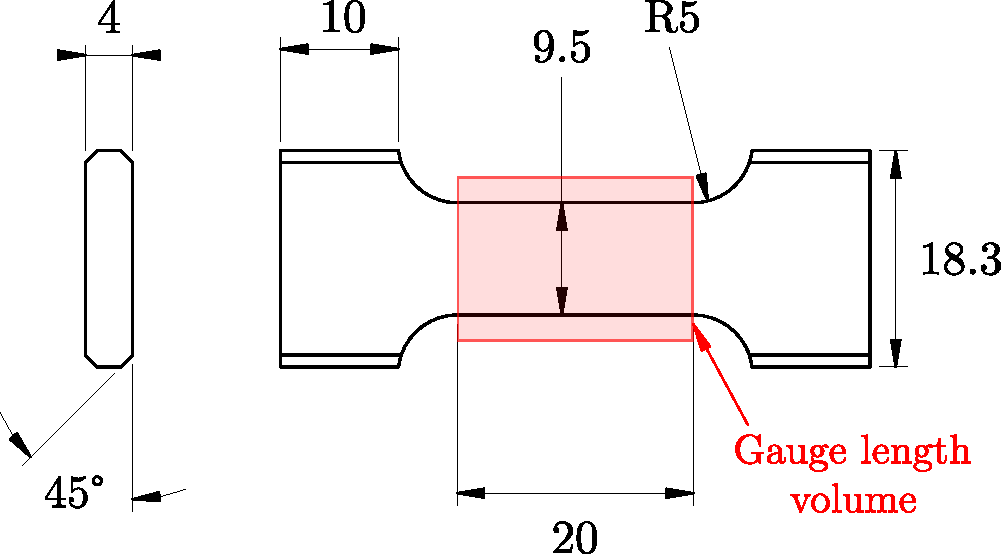
\includegraphics[width=0.9\textwidth]{Images/TDS_specimen.pdf} \\
%	\end{figure}
%\end{column}
%
%\end{columns}
%
%\end{frame}
%
%%%%%%%%%%%%%%%%%%%%%%%%%%%%%%%%%%%%%%%%%%%%%%%%%%%%%%%%%%%%
%
%\begin{frame}{Experimental procedure}
%
%\textbf{\textcolor{MINESBlue}{\large Thermal Desorption Spectroscopy (TDS) test:}}
%\vspace{0.15cm}
%\begin{itemize}
%	\item High precision (10$^{-3}$ wppm), calibration with a Certified Reference Material (CRM) with a known hydrogen mass
%	\vspace{0.15cm}
%	\item Temperature ramp of 10$^{\circ}$C/min up to 600$^{\circ}$C 
%	\vspace{0.15cm}
%	\item The hydrogen content is determined by integrating the first peak in the TDS spectra
%\end{itemize}
%
%\begin{figure}
%	\centering
%	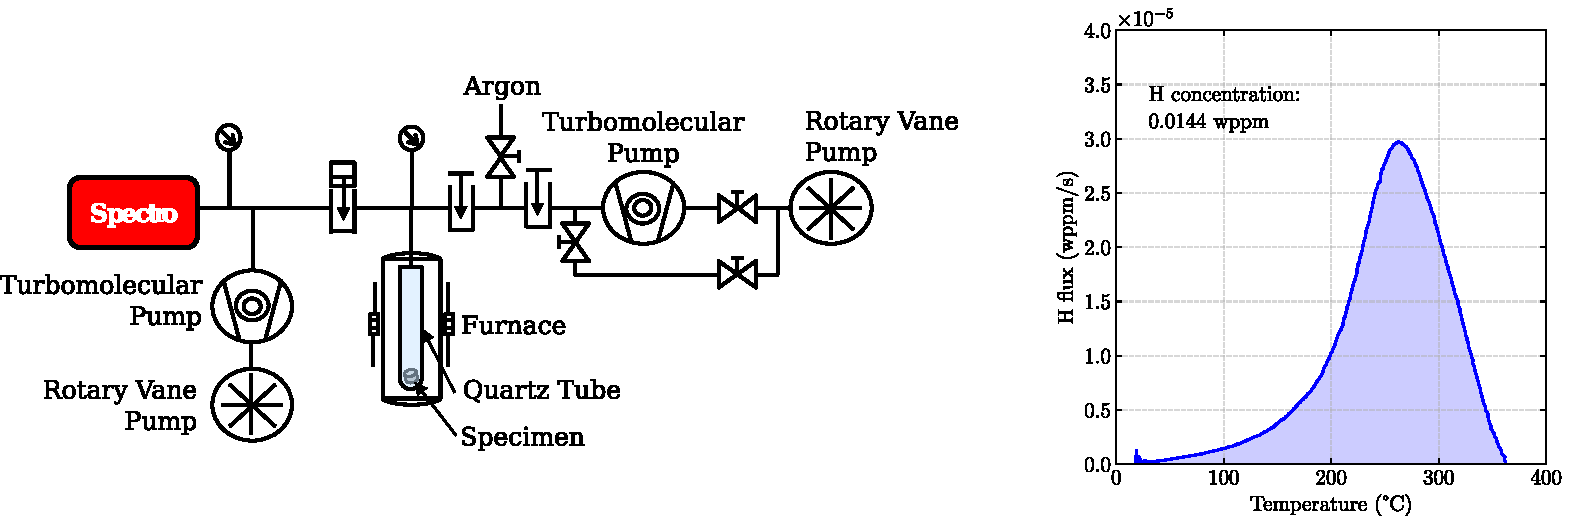
\includegraphics[width=0.95\textwidth]{Images/TDS_spectra.pdf} \\
%\end{figure}
%
%\end{frame}
%
%%%%%%%%%%%%%%%%%%%%%%%%%%%%%%%%%%%%%%%%%%%%%%%%%%%%%%%%%%%%
%
%\begin{frame}{Simulation model}
%
%\begin{columns}
%
%\begin{column}{0.65\textwidth}
%
%\begin{itemize}
%	\item 3D mesh of 1/8 of the specimen (plane strain)
%	\vspace{0.15cm}
%	\item Elasto(visco)-plastic behavior
%	\vspace{0.15cm}
%	\item Hydrogen applied to the exposed surfaces
%	\vspace{0.15cm}
%	\item $N_T(\kappa)$ adjusted based on experimental results at different strain levels
%\end{itemize}
%
%	\vspace{0.25cm}
%
%	\begin{figure}
%		\centering
%		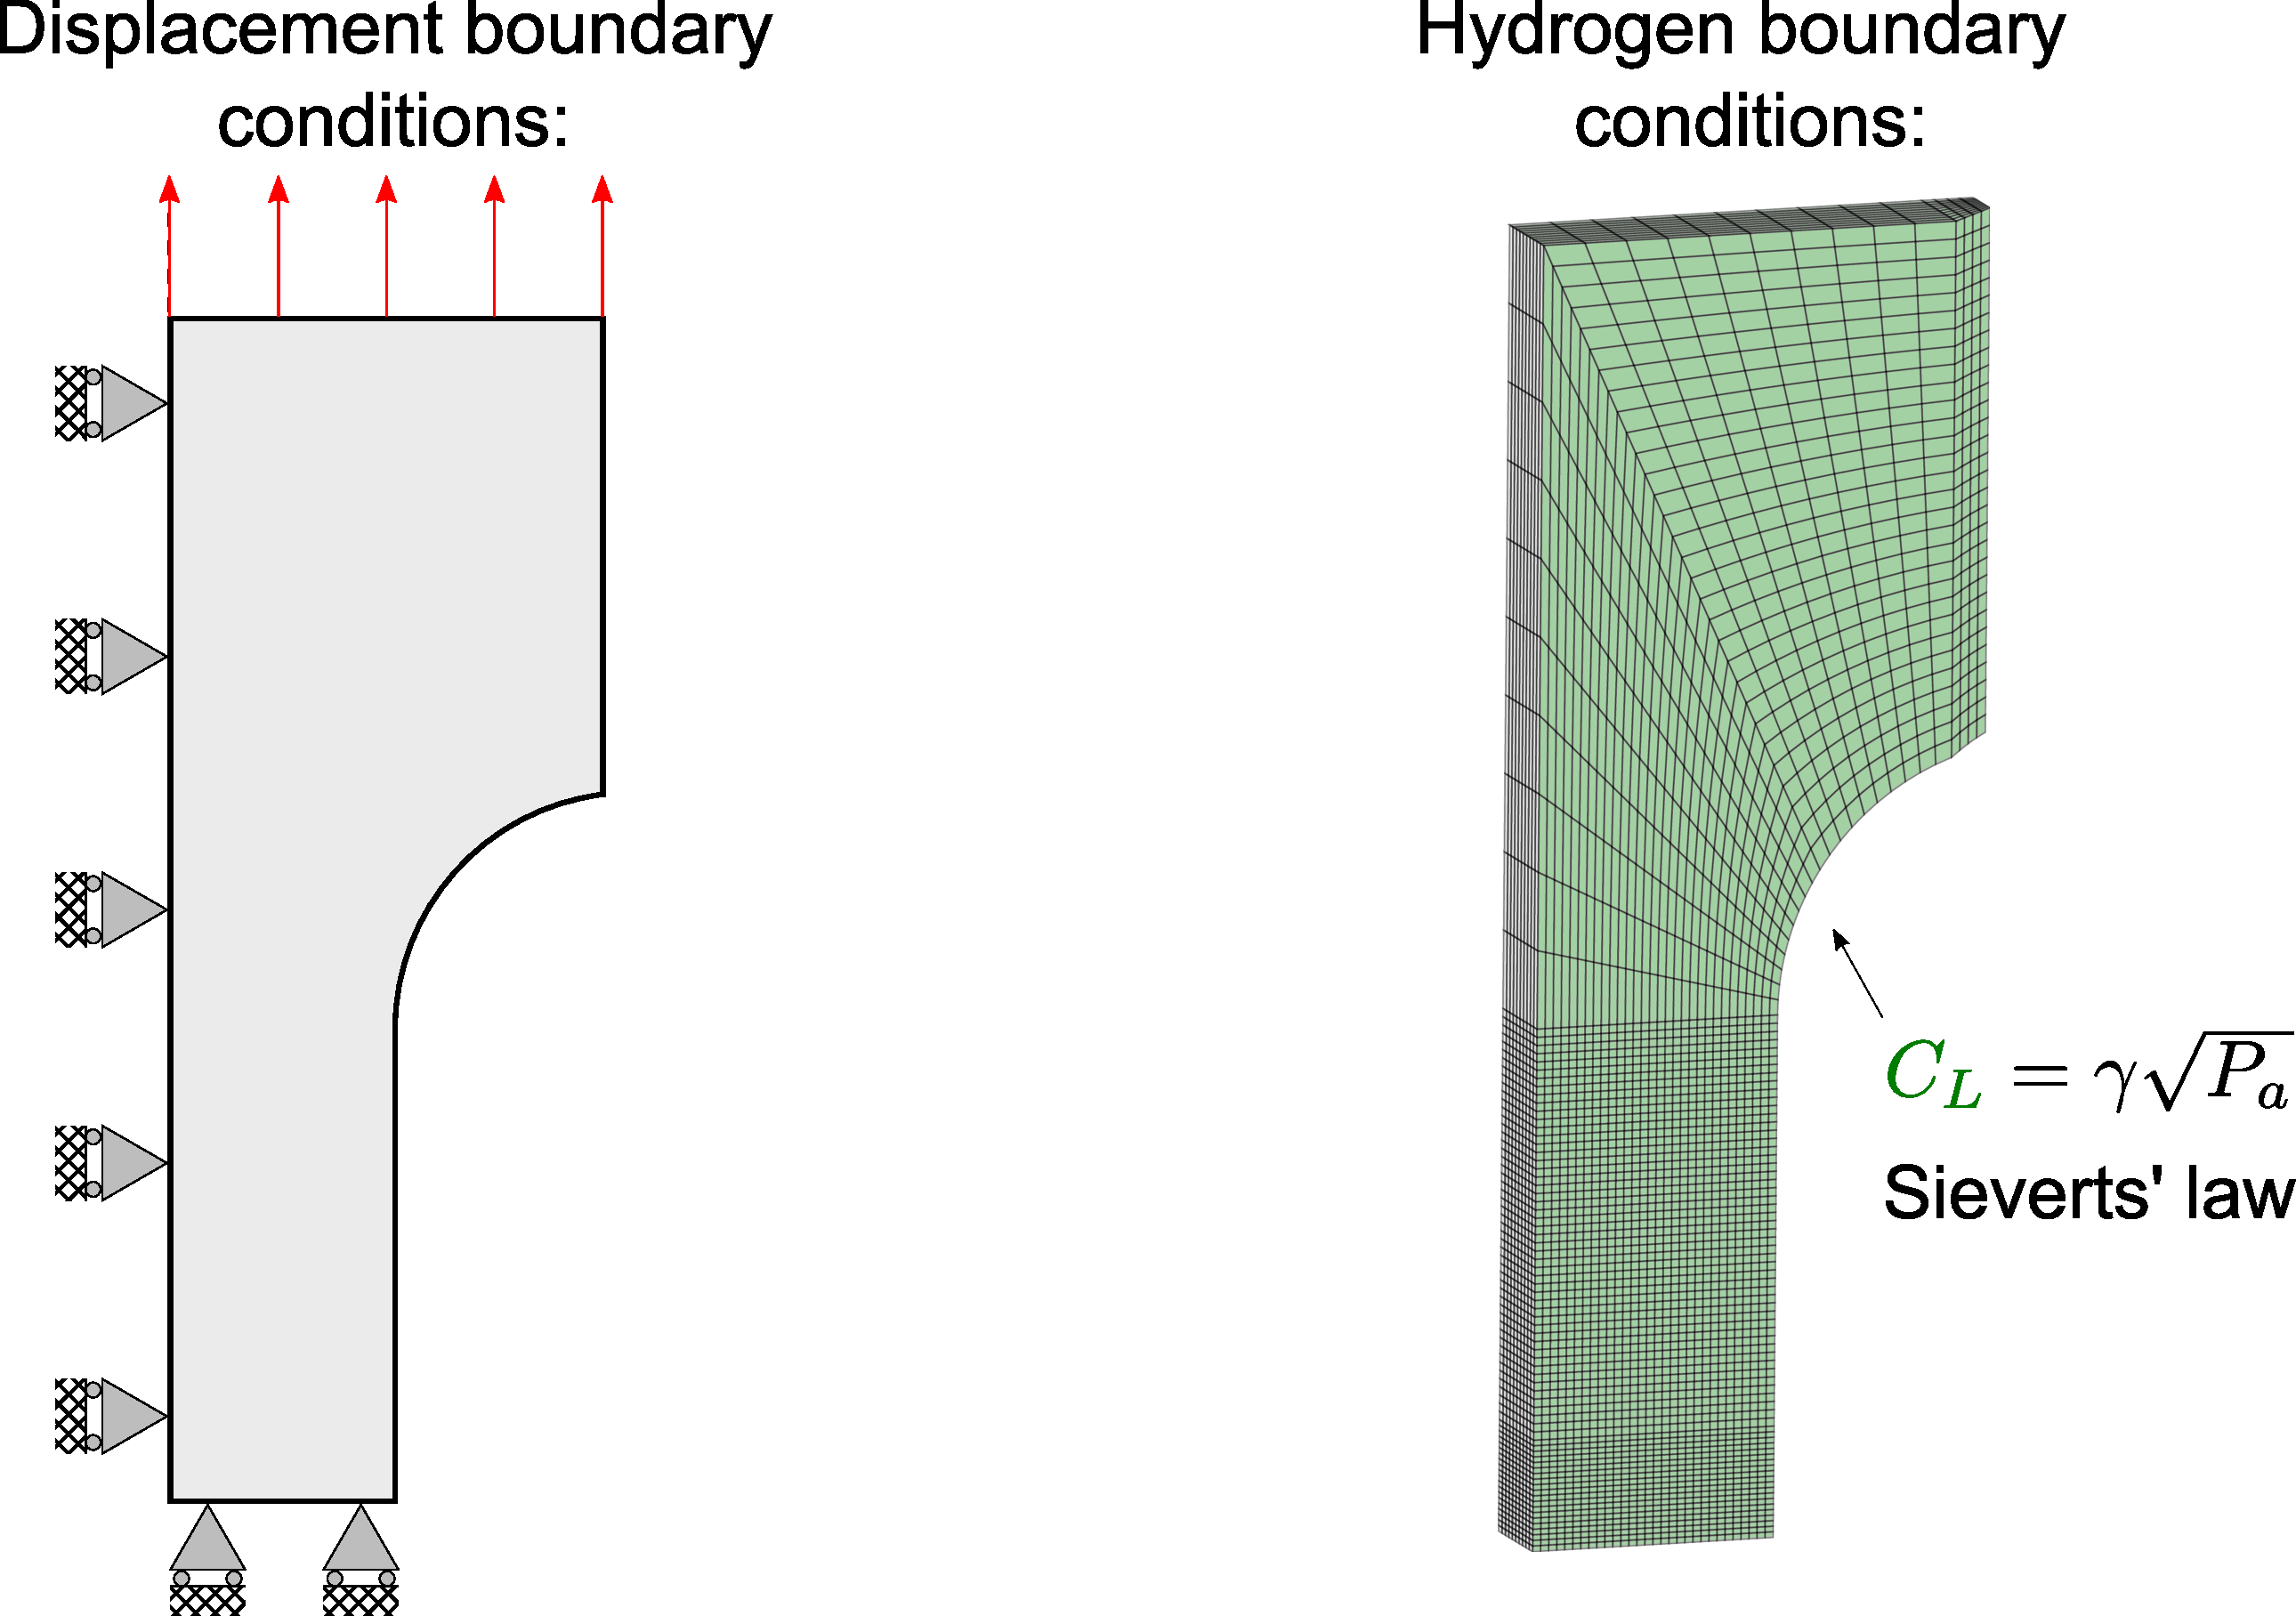
\includegraphics[width=0.8\textwidth]{Images/TDS_BC.pdf} \\
%	\end{figure}
%	
%	\vspace{0.15cm}
%
%\end{column}
%
%\begin{column}{0.35\textwidth}
%	\begin{figure}
%		\centering
%		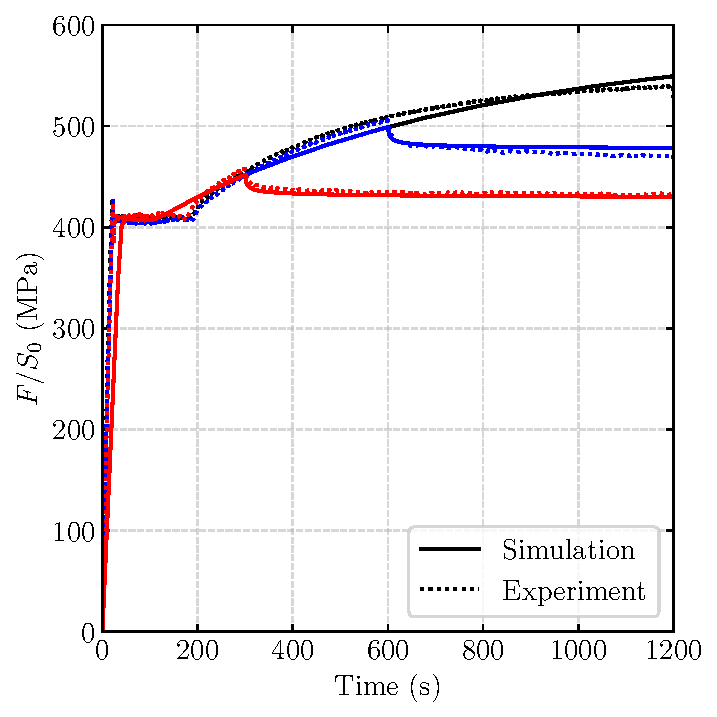
\includegraphics[width=0.99\textwidth]{Images/plot_time_stress.pdf} \\
%		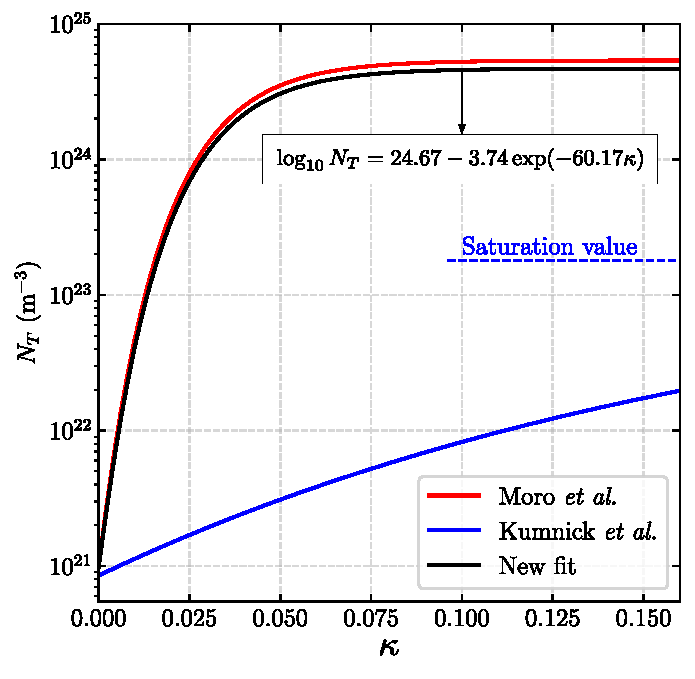
\includegraphics[width=0.95\textwidth]{Images/NT_TDS.pdf}
%	\end{figure}
%\end{column}
%
%\end{columns}
%
%\end{frame}
%
%%%%%%%%%%%%%%%%%%%%%%%%%%%%%%%%%%%%%%%%%%%%%%%%%%%%%%%%%%%%
%
%\begin{frame}{Strain effect}
%
%\begin{itemize}
%	\item Specimens deformed up to 90\%Rp02, 3\%, 6\% and 12\% at 
%	$\dot{\varepsilon} = 1\times10^{-4}$ s$^{-1}$
%	\vspace{0.15cm}
%	\item Higher strain levels lead to higher hydrogen concentrations
%	\vspace{0.15cm}
%	\item Most of hydrogen is located at the gauge length
%	\vspace{0.15cm}
%	\item For all cases, hydrogen is mostly located near the surface
%\end{itemize}
%
%\vspace{0.15cm}
%
%	\begin{figure}
%		\centering
%		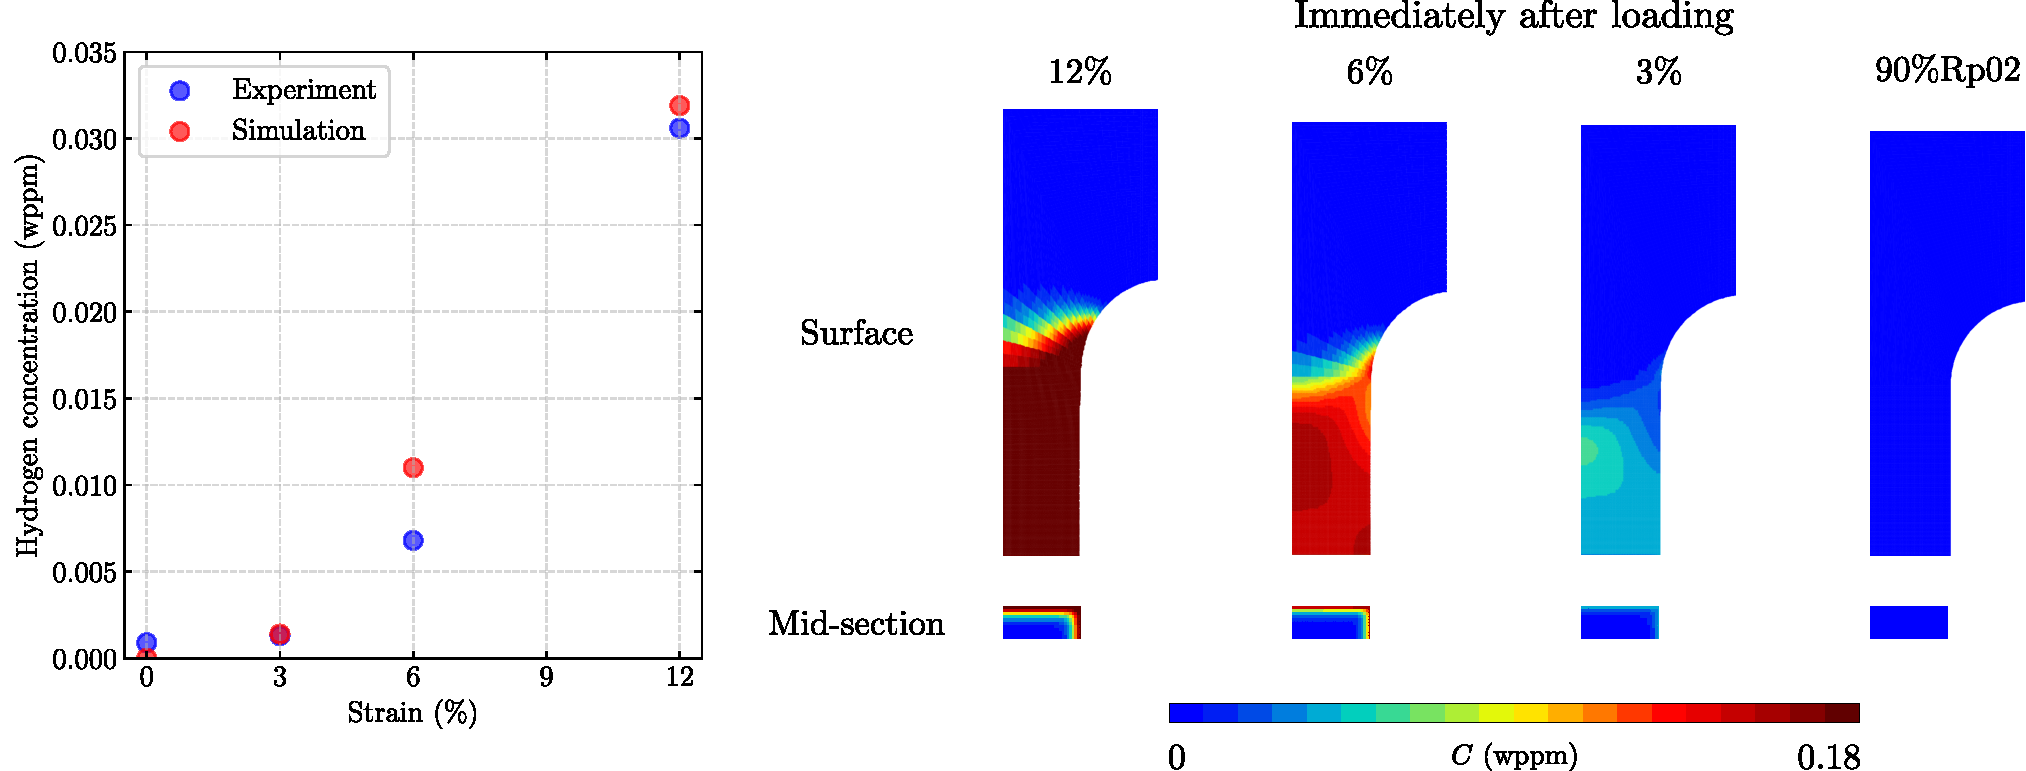
\includegraphics[width=\textwidth]{Images/strain_effect.pdf} \\
%	\end{figure}
%
%\end{frame}
%
%%%%%%%%%%%%%%%%%%%%%%%%%%%%%%%%%%%%%%%%%%%%%%%%%%%%%%%%%%%%
%
%\begin{frame}{Strain effect}
%
%	\begin{itemize}
%		\item The preparations required before the TDS test takes approximately \textbf{one hour}, at which hydrogen can freely desorb the specimen
%		\vspace{0.15cm}
%		\item The amount of hydrogen that leaves the specimen during resting is lower at higher strains
%		\vspace{0.15cm}
%		\item With the actual model, at least 80\% of the hydrogen content leaves the specimen during resting
%	\end{itemize}
%
%	\begin{figure}
%		\centering
%		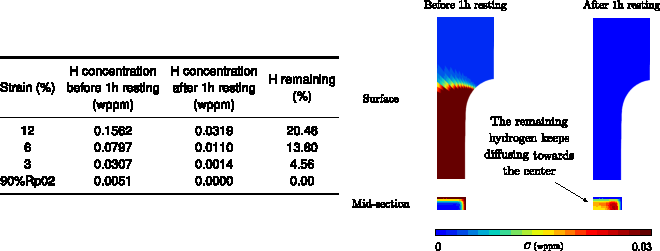
\includegraphics[width=\textwidth]{Images/resting_time.pdf} \\
%	\end{figure}
%
%\end{frame}
%
%
%%%%%%%%%%%%%%%%%%%%%%%%%%%%%%%%%%%%%%%%%%%%%%%%%%%%%%%%%%%%
%
%\begin{frame}{Strain rate effect}
%
%\begin{columns}
%
%\begin{column}{0.55\textwidth}
%\begin{itemize}
%	\item Tests conducted at three different strain rates: $1\times10^{-3}$, $1\times10^{-4}$ and $1\times10^{-5}$ s$^{-1}$
%	\vspace{0.25cm}
%	\item One-hour resting time allowing hydrogen desorption is considered
%	\vspace{0.25cm}
%	\item \textbf{Lower strain rates} lead to \textbf{higher hydrogen content}, as hydrogen has more time to diffuse throughout the material
%\end{itemize}
%\end{column}
%
%\begin{column}{0.45\textwidth}
%\begin{figure}
%	\centering
%	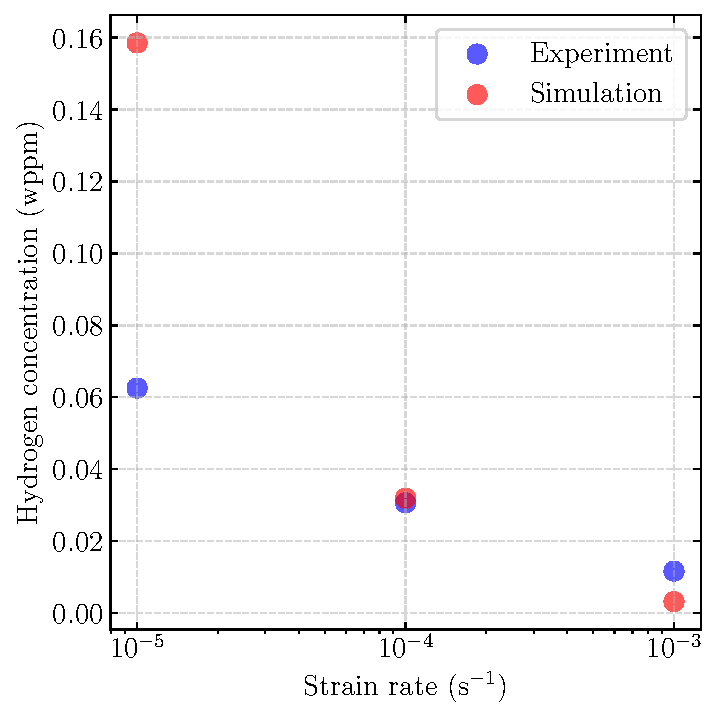
\includegraphics[width=0.9\textwidth]{Images/strain_rate_effect.pdf} \\
%	\vspace{0.25cm}
%%	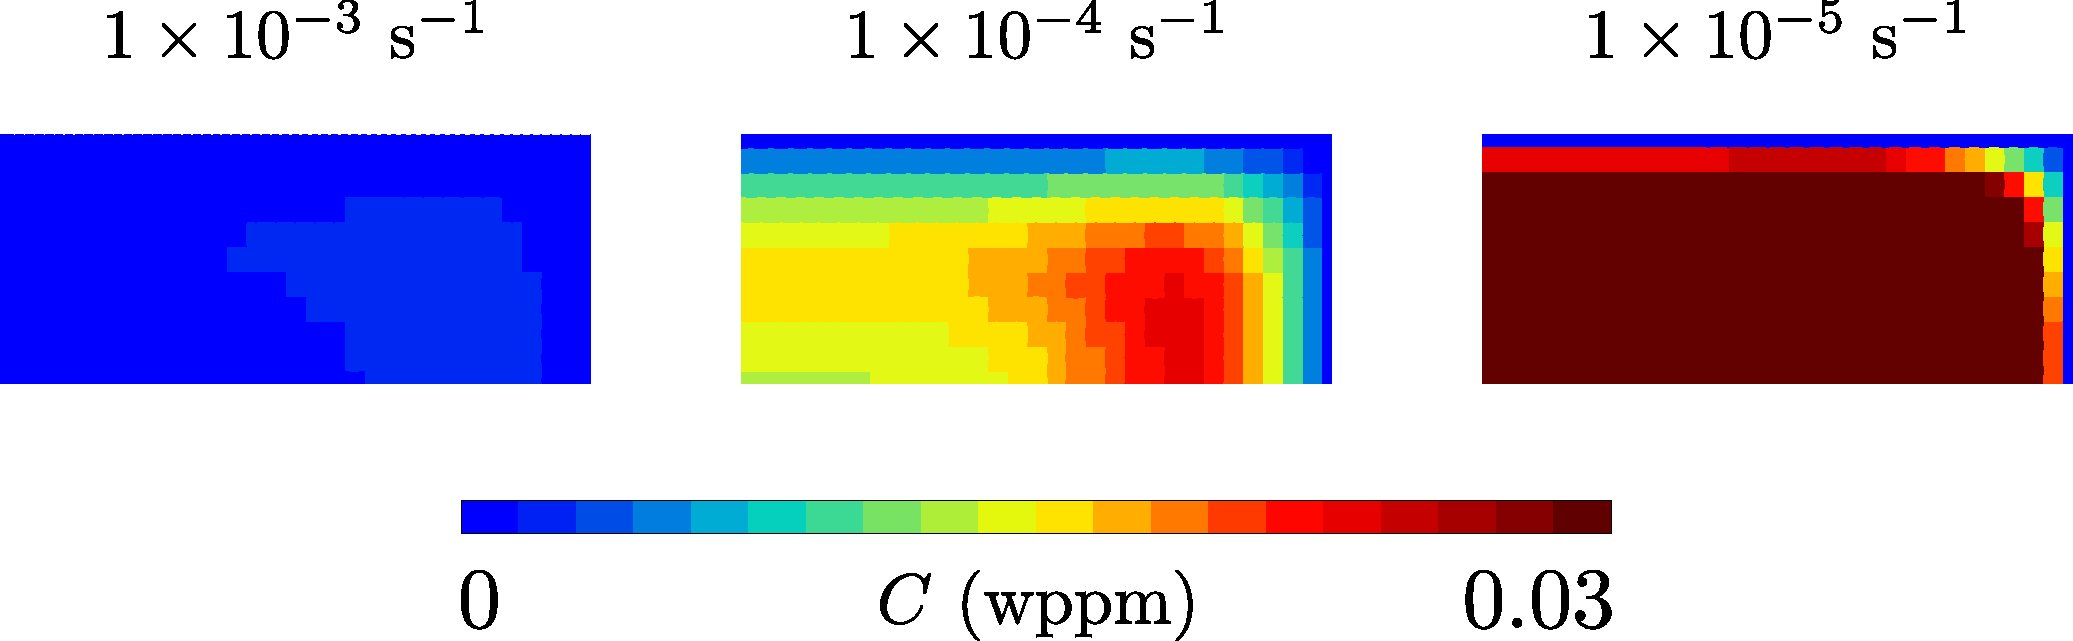
\includegraphics[width=\textwidth]{Images/C_field_strain_rate_effect.pdf}
%\end{figure}
%
%\end{column}
%\end{columns}
%
%\begin{figure}
%		\centering
%		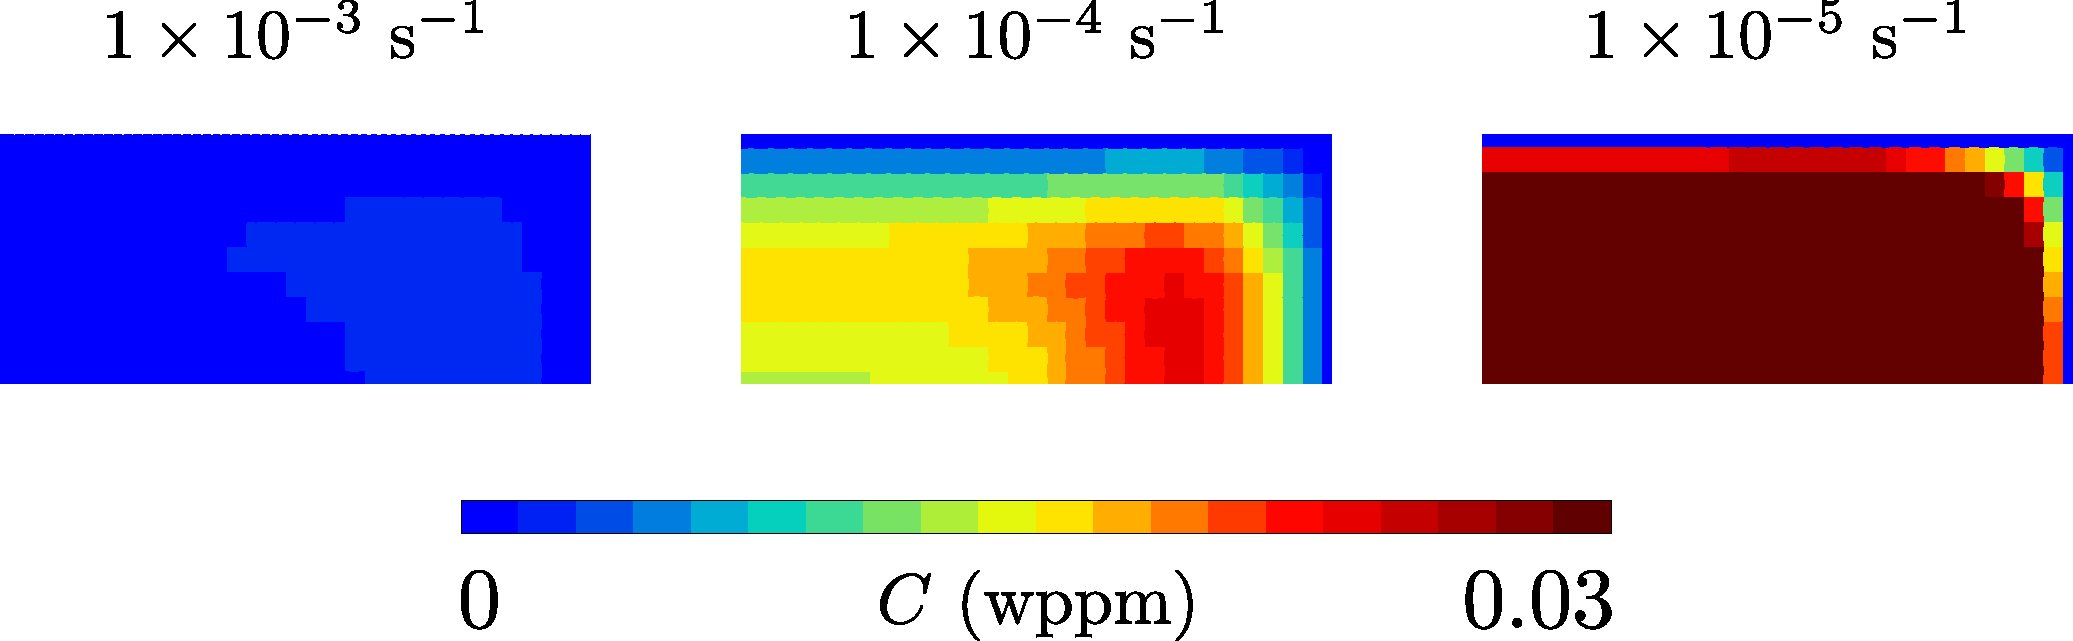
\includegraphics[width=0.65\textwidth]{Images/C_field_strain_rate_effect.pdf} \\
%	\end{figure}
%
%\end{frame}
%
%%%%%%%%%%%%%%%%%%%%%%%%%%%%%%%%%%%%%%%%%%%%%%%%%%%%%%%%%%%%
%
%\begin{frame}{Dwell effect}
%
%\begin{itemize}
%	\item \textbf{Dwell time:} the time a specimen is exposed to hydrogen without further deformation until it reaches the same exposure time as the most deformed specimen (12\%)
%	\vspace{0.25cm}
%	\item Specimens deformed up to 3\% strain at $1\times10^{-4}$ $1\times10^{-5}$ s$^{-1}$
%	\vspace{0.25cm}
%	\item Longer exposure $\rightarrow$ Higher hydrogen content
%\end{itemize}
%
%\begin{figure}
%	\centering
%	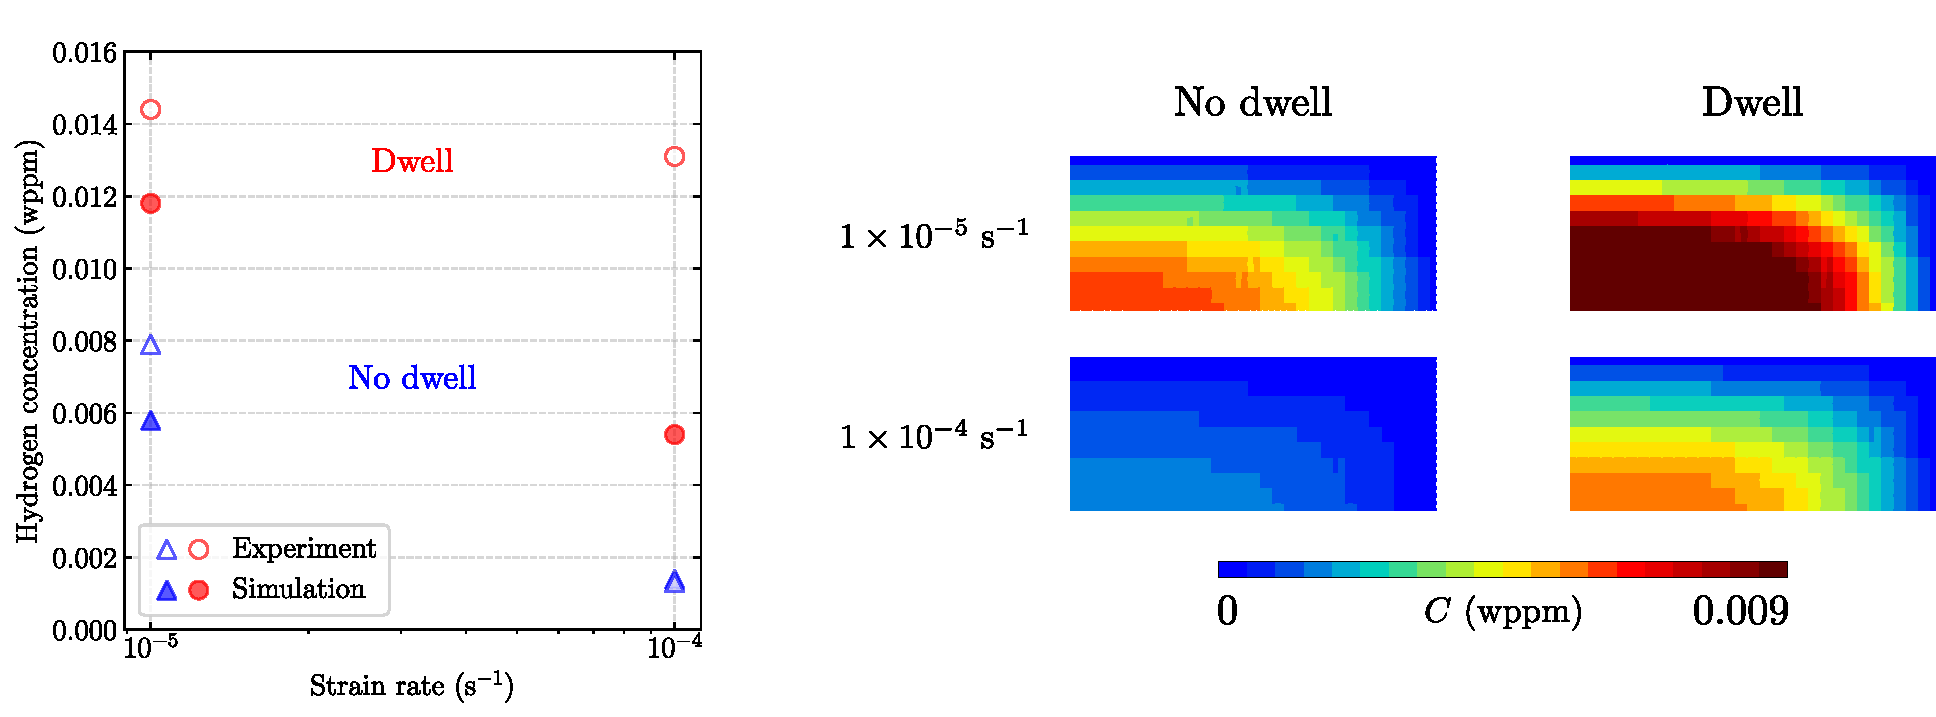
\includegraphics[width=\textwidth]{Images/Dwell_No_Dwell.pdf} 
%\end{figure}
%
%\end{frame}

%%%%%%%%%%%%%%%%%%%%%%%%%%%%%%%%%%%%%%%%%%%%%%%%%%%%%%%%%%%

\subsection{Hydrogen embrittlement modeling}

\begin{frame}{Outline}
	\tableofcontents[ 
    currentsubsection, 
    hideothersubsections, 
    sectionstyle=show/shaded, 
    subsectionstyle=show/shaded, 
    ] 
\end{frame}

%%%%%%%%%%%%%%%%%%%%%%%%%%%%%%%%%%%%%%%%%%%%%%%%%%%%%%%%%%%

\begin{frame}{Database and material coefficients}

    \begin{itemize}
        \item \textbf{Database}: Briottet \textit{et al.}, 2012 and Moro \textit{et al.}, 2010: \textit{Effect of gaseous hydrogen on the mechanical properties of steel}
        
        \vspace{0.15cm}

        \item \textbf{Material:} high-strength steel (API X80 grade) in an environment of hydrogen and neutral gas
        
        \vspace{0.15cm}   

    \end{itemize}
    
\begin{columns}

	\begin{column}{0.6\textwidth}

	\begin{itemize}

		\item As HE corresponds to \textbf{quasi-cleavage}, a \textbf{stress dependance} is introduced to the nucleation law
                
		\vspace{0.15cm}
                
        \item The function expressing the nucleation rate due to quasi-cleavage is:
                
		\begin{equation*}
                    \textcolor{NewRed}{B_n(C)} = \frac{\textcolor{DarkGreen}{B_0}}{\textcolor{DarkGreen}{\sigma_C^0}} (\sigma_I - (1-q_1 f_{*})\textcolor{blue}{\sigma_C})
		\end{equation*}

		\vspace{0.15cm}

		\item Hydrogen decreases the critical stress to trigger void nucleation
        
	\end{itemize}

	\end{column}
    
    \begin{column}{0.4\textwidth}

	\begin{figure}
		\begin{tabular}{c}
			\includegraphics[width=0.95\textwidth]{Images/plot_sig_c.pdf}
		\end{tabular}
	\end{figure}

	\begin{textblock}{5}(11.5,14.15)
		\textcolor{DarkGreen}{\footnotesize (Material parameters)}
	\end{textblock}

	\end{column}
    
\end{columns}

\end{frame}

%%%%%%%%%%%%%%%%%%%%%%%%%%%%%%%%%%%%%%%%%%%%%%%%%%%%%%%%%%%

\begin{frame}{Tensile tests}

    \begin{itemize}
        \item Tensile tests under different strain rates under hydrogen gas
        \vspace{0.15cm}
        \item Slower rates lead to important ductility losses
    \end{itemize}
    
    \begin{columns}
    
        \begin{column}{0.45\textwidth}
            \begin{figure}
                \begin{tabular}{c}
                    \includegraphics[width=0.9\textwidth]{Images/ST_specimen_Moro_BC.pdf}\\
                    \\
                    \includegraphics[width=0.8\textwidth]{Images/fracture_surface.png}\\
                \end{tabular}
            \end{figure}
            \centering \scriptsize \textcolor{gray}{(Experimental data: Briottet \textit{et al.}, 2012)}
        \end{column}
    
    
        \begin{column}{0.55\textwidth}
            \begin{figure}
                \begin{tabular}{c}
                    \includegraphics[width=0.6\textwidth]{Images/calcul_pl.pdf}\\
                    \\
                    \includegraphics[width=0.7\textwidth]{Images/fig_ST_sim_edt.pdf}\\
                \end{tabular}
            \end{figure} 
        \end{column}
    
    \end{columns}
    
\end{frame}

%%%%%%%%%%%%%%%%%%%%%%%%%%%%%%%%%%%%%%%%%%%%%%%%%%%%%%%%%%%

\begin{frame}{Tensile tests}

    \begin{itemize}
        \item Different damage evolution under hydrogen environment
        \vspace{0.15cm}
        \item Multicrack initiation on the surface
    \end{itemize}

    \vspace{4.5cm}

% ------------------------------------------------

\begin{tikzpicture}[remember picture, overlay]
    \node at (current page.south west) [xshift=4.5cm, yshift=4cm] {\includegraphics[width=0.7\textwidth]{Images/fig_ST_f_edt.pdf}}; 
\end{tikzpicture}

% ------------------------------------------------

    \begin{tikzpicture}[remember picture, overlay]
    
        \node at (current page.south west) [xshift=10.9cm, yshift=4.15cm]{
            \includemedia[
            % width=0.8\linewidth,height=0.6\linewidth, 
            width=0.3\textwidth,
            activate=onclick,
            passcontext, % Keep the \pause, etc. working in overlays
            addresource=Images/anim_surf_cracks/output.mp4, % chemin de votre fichier vidéo
            flashvars={
                source=Images/anim_surf_cracks/output.mp4   % chemin de votre fichier vidéo
                &autoPlay=true     % autoplay de la vidéo
                &loop=true         % lire en boucle
            }
        ]{\includegraphics[width=0.3\textwidth]{Images/anim_surf_cracks/anim0159.png}}{VPlayer.swf}};
    
    \end{tikzpicture}

\end{frame}

%%%%%%%%%%%%%%%%%%%%%%%%%%%%%%%%%%%%%%%%%%%%%%%%%%%%%%%%%%%

\begin{frame}{Pressurized disk tests}
    \textbf{Hydrogen effect:}

    \vspace{0.2cm}

    \begin{itemize}
        \item Lower pressure at rupture with decreased ductility
        \vspace{0.15cm}
        \item Higher hydrogen concentration in the rupture zone
    \end{itemize}

    \vspace{0.1cm}

    \begin{columns}

        \begin{column}{0.45\textwidth}

            \begin{figure}
                \begin{tabular}{c}
                    \includegraphics[width=0.9\textwidth]{Images/fig_disk_tP.pdf}\\
                \end{tabular}
            \end{figure}

        \end{column}
    
        \begin{column}{0.55\textwidth}
            \begin{figure}
                \begin{tabular}{c}
                    \includegraphics[width=0.9\textwidth]{Images/fig_iso_values_disk.pdf}\\
                \end{tabular}
            \end{figure}
        \end{column}
    
    \end{columns}
    
\end{frame}

%%%%%%%%%%%%%%%%%%%%%%%%%%%%%%%%%%%%%%%%%%%%%%%%%%%%%%%%%%%

\begin{frame}{Pressurized disk tests}

    \textbf{Effect of the pressurization rate:}
    \vspace{0.15cm}

    \begin{itemize}
        \item Tests under different pressurization rates on H$_{\textrm{e}}$ and H$_2$ gases
        \vspace{0.15cm}
        \item \textbf{Lower pressurization rate} $\rightarrow$ \textbf{Higher embrittlement} since has a longer time to diffuse
    \end{itemize}

    \begin{columns}

        \begin{column}{0.45\textwidth}

            \begin{figure}
                \begin{tabular}{c}
                    \includegraphics[width=0.9\textwidth]{Images/fig_disk_Pr_edt.pdf}\\
                \end{tabular}
            \end{figure}

            \centering \hspace{0.8cm} \scriptsize \textcolor{gray}{(Experimental data: Briottet \textit{et al.}, 2012)}

        \end{column}
    
        \begin{column}{0.55\textwidth}
            \begin{figure}
                \begin{tabular}{c}
                    \includegraphics[width=0.9\textwidth]{Images/C_P_rate.pdf}\\
                \end{tabular}
            \end{figure}
        \end{column}
    
    \end{columns}   
    
\end{frame}

%%%%%%%%%%%%%%%%%%%%%%%%%%%%%%%%%%%%%%%%%%%%%%%%%%%%%%%%%%%

\begin{frame}{Fracture toughness tests}


    \begin{itemize}
        \item 2D Compact Tension (CT) specimen - \textit{plane strain}
        \vspace{0.1cm}
        \item Uniaxial imposed displacement
        \vspace{0.1cm}
        \item Environment: air and hydrogen (30 MPa)
        \vspace{0.1cm}
        \item Lattice concentration (\textcolor{DarkGreen}{$C_L$}) derived from Sieverts' law imposed on the newly formed crack
    \end{itemize}

    \vspace{0.25cm}

    \begin{columns}

        \begin{column}{0.4\textwidth}

            \begin{figure}
                \begin{tabular}{c}
                    \includegraphics[width=0.85\textwidth]{Images/CT_specimen.pdf}\\
                \end{tabular}
            \end{figure}

        \end{column}
    
        \begin{column}{0.6\textwidth}

        \begin{figure}
            \begin{tabular}{c}
                \includegraphics[width=0.9\textwidth]{Images/CT_BC.pdf}\\
            \end{tabular}
        \end{figure}

        \end{column}
    
    \end{columns}  

\end{frame}

%%%%%%%%%%%%%%%%%%%%%%%%%%%%%%%%%%%%%%%%%%%%%%%%%%%%%%%%%%%

\begin{frame}{Fracture toughness tests}

    \begin{itemize}
        \item Crack length: post-processing considering broken elements $f_* = 0.99 \times 1/q_1$
        \vspace{0.15cm}
        \item $J$ computation: ASTM E1820 standard considering the simulated Load-CMOD curve
    \end{itemize}

\vspace{5cm}

% --------------------------------------------------

\begin{tikzpicture}[remember picture, overlay]
    \node at (current page.south west) [xshift=3.cm, yshift=3.25cm] {\includegraphics[width=5.5cm]{Images/J_da.pdf}}; 
\end{tikzpicture}

% --------------------------------------------------

\begin{tikzpicture}[remember picture, overlay]
    
    \node at (current page.south west) [xshift=9.5cm, yshift=3.4cm]{
        \includemedia[
        width=0.55\textwidth,
        activate=onclick,
        passcontext, % Keep the \pause, etc. working in overlays
        addresource=Images/anim_CT/output.mp4, % chemin de votre fichier vidéo
        flashvars={
            source=Images/anim_CT/output.mp4   % chemin de votre fichier vidéo
            &autoPlay=true     % autoplay de la vidéo
            &loop=true         % lire en boucle
        }
    ]{\includegraphics[width=0.55\textwidth]{Images/anim_CT/anim00.png}}{VPlayer.swf}};

\end{tikzpicture}
    
\end{frame}

%%%%%%%%%%%%%%%%%%%%%%%%%%%%%%%%%%%%%%%%%%%%%%%%%%%%%%%%%%%

\subsection{Simulation of fracture toughness tests}

\begin{frame}{Outline}
	\tableofcontents[ 
    currentsubsection, 
    hideothersubsections, 
    sectionstyle=show/shaded, 
    subsectionstyle=show/shaded, 
    ] 
\end{frame}


%%%%%%%%%%%%%%%%%%%%%%%%%%%%%%%%%%%%%%%%%%%%%%%%%%%%%%%%%%%

\section{Conclusions and perspectives}

\begin{frame}{Outline}
	\tableofcontents[ 
    currentsubsection, 
    hideothersubsections, 
    sectionstyle=show/shaded, 
    subsectionstyle=show/shaded, 
    ] 
\end{frame}

%%%%%%%%%%%%%%%%%%%%%%%%%%%%%%%%%%%%%%%%%%%%%%%%%%%%%%%%%%%

\section*{}

\begin{frame}{}

    \begin{columns}

        \begin{column}{0.6\textwidth}
            \begin{figure}
                \begin{tabular}{c}
                    \includegraphics[width=0.6\textwidth]{TEMPLATE_IMAGES/MINES.png} \\
                \end{tabular}
            \end{figure}
        \end{column}

        \begin{column}{0.4\textwidth}
            \begin{figure}
                \begin{tabular}{c}
                    \includegraphics[width=0.5\textwidth]{TEMPLATE_IMAGES/MESSIAH.pdf} \\
                \end{tabular}
            \end{figure}
        \end{column}

    \end{columns}

    \vspace{0.5cm}

    \noindent\makebox[\linewidth]{\rule{1.0\textwidth}{0.4pt}}

    \vspace{0.3cm}

    \begin{center}
        \Huge{\textcolor{MINESBlue}{\textbf{Thank you}}} \\
        \vspace{1.0cm}
        \normalsize Daniella LOPES PINTO \\
        \vspace{0.1cm}
        \small \texttt{\textcolor{black}{daniella.lopes\_pinto@minesparis.psl.eu}}
    \end{center}

    \vspace{0.3cm}

    \noindent\makebox[\linewidth]{\rule{1.0\textwidth}{0.4pt}}

    \begin{figure}
        \begin{tabular}{c}
            \includegraphics[width=1.0\textwidth]{TEMPLATE_IMAGES/logos_MESSIAH.pdf} \\
        \end{tabular}
    \end{figure}

\end{frame}

\end{document}